\documentclass[11pt]{ujarticle}
%\documentclass{jlreq,11pt}
%%%%%%% スタイルファイル %%%%%%%%%%%%%%%%%%%%%%
\usepackage{lmodern}
\usepackage{amsmath,amssymb}

\usepackage{thesis}

\usepackage[dvipdfmx]{graphicx}   % pdf 形式の図版取り込みのため
\usepackage{ascmac}
\usepackage{multicol}
\usepackage{array}
\usepackage{float}
\usepackage{indent}
\setlength{\parindent}{1em} % 段落の字下げを2文字分にする

\usepackage{url}

\usepackage{color}
\definecolor{lightgray}{gray}{0.9}
\definecolor{darkgray}{gray}{0.25}

\usepackage{framed}
\makeatletter
\renewenvironment{leftbar}{%
  \def\FrameCommand{\hspace{1.5zw}\textcolor{darkgray}{\vrule width 2pt}\hspace{0.5zw}}% 
  \MakeFramed {\advance\hsize-\width \FrameRestore}}%
 {\endMakeFramed}
\makeatother


\usepackage{listings,jvlisting} 
\usepackage{xcolor} % 必要なら色をつけるため
\usepackage{caption}
%\captionsetup[lstlisting]{labelfont=bf, font=footnotesize, format=plain, singlelinecheck=false}

\lstset{
    basicstyle=\ttfamily\scriptsize,      % フォントサイズとスタイル
    keywordstyle=\color{blue},            % キーワードの色
    commentstyle=\color{green},           % コメントの色
    stringstyle=\color{red},              % 文字列の色
    numbers=left,                         % 行番号を左側に表示
    stepnumber=1,                         % 行番号の間隔
    numbersep=10pt,                       % 行番号とコードの間隔
    frame=tb,                             % 上下に枠を表示
    captionpos=b,                         % キャプションの位置を下
    breaklines=true,                      % 長い行を折り返す
    breakatwhitespace=false,              % 空白で改行しない
    showspaces=false,                     % スペースを表示しない
    showstringspaces=false,               % 文字列中のスペースを表示しない
    tabsize=4,                            % タブ幅
    extendedchars=true,                   % 拡張文字セットを有効化(日本語対応)
    inputencoding=utf8,                   % 入力文字エンコーディングをUTF-8に設定
    backgroundcolor={\color[gray]{.95}},  %背景の色設定    
}



\begin{document}

%%%%%%%%%%%%%%%%%%%%%%%%%%%%%%%%%%%%%%%%%%%%%%%%%%%%%%%%%%%%%%%%%%%%%%%%%%%%%
%%%%%% 表紙 %%%%%%%%%%%%%%%%%%%%%%%%%%%%%%%%%%%%%%%%%%%%%%%%%%%%%%%%%%%%%%%
%%%%%%%%%%%%%%%%%%%%%%%%%%%%%%%%%%%%%%%%%%%%%%%%%%%%%%%%%%%%%%%%%%%%%%%%%%%%%

% === 年度を記入 ============================================================
\def\year{5}	% 令和 1 年度の場合

% === 提出年月日を記入 ============================================================
\def\submityear{2}	% 令和 2 年
\def\submitmonth{2}	% 2 月
\def\submitdate{4}	% 4 日

% === 題目を記入 ============================================================
\def\title{%
  人追従搬送ロボットのシステム開発
}%

% === 題目を記入(背表紙用) ============================================================
\def\spine{%
  人追従搬送ロボットのシステム開発
}%

% === 学科を記入 ==========================================================
\def\course{電子制御工学科}

% === 学籍番号を記入 ========================================================
\def\student_number{s9123}

% === 氏名を記入 ============================================================
\def\name{野口 史遠}

% === 指導教員を記入 ========================================================
\def\supervisor{{高木 太郎 教授}}

% === 表紙 ========================================================
\thispagestyle{empty}
% !TEX root = main.tex


{\renewcommand{\arraystretch}{0.5}
\begin{tabular}{|p{16.5cm}|}
\hline
{\scriptsize{舞鶴工業高等専門学校 電子制御工学科 卒業論文 (令和\ \submityear\ 年\ \submitmonth\ 月\ \submitdate\ 日提出)}}\\
{\small\bf{\spine}}\\
\hfill\scriptsize\bf{\name (\student_number)}
\\
\hline
\end{tabular}}

\newpage
% ======================================================================
\begin{center}
{\fontsize{20pt}{0pt}\selectfont\bf{令和\ \year\ 年度}}\\[1zh]
{\fontsize{28pt}{0pt}\selectfont\bf{\kintou{8zw}{卒業研究論文}}}
\end{center}
% ======================================================================
\vspace{2zh}


% ======================================================================
\begin{center}
\fontsize{20pt}{26pt}\selectfont
\renewcommand{\arraystretch}{1.4}
\begin{tabular}{|p{2zw}|p{20zw}|}
\hline
{\bf{題目}} &
{\bf{\title}}\\\hline
\end{tabular}
\end{center}
% ======================================================================
\vspace{2zh}

% ======================================================================
\begin{center}
\fontsize{16pt}{18pt}\selectfont
\renewcommand{\arraystretch}{1.4}
\tabcolsep 4pt
\begin{tabular}{|p{4zw}|p{14zw}|}
\hline
{\bf{\kintou{4zw}{学科}}} &
{\bf{\course}}\\\hline
{\bf{\kintou{4zw}{学籍番号}}} &
{\bf{\student_number}}\\\hline
{\bf{\kintou{4zw}{氏名}}} &
{\bf{\name}}\\\hline
{\bf{\kintou{4zw}{提出日}}} &
{\bf{令和\ \submityear\ 年\ \submitmonth\ 月\ \submitdate\ 日}}\\\hline
\end{tabular}
\end{center}
% ======================================================================
\vspace{0zh}

% ======================================================================
\begin{center}
\fontsize{16pt}{18pt}\selectfont
\renewcommand{\arraystretch}{1.4}
\tabcolsep 4pt
\begin{tabular}{|p{4zw}|p{14zw}|}
\hline
{\bf{\kintou{4zw}{指導教員}}} &
{\bf{\supervisor}}\\\hline
\end{tabular}
\end{center}
% ======================================================================

\vfill
% ======================================================================
\begin{center}

\includegraphics[width=45mm]{figure/logo_maizuru_gray.pdf}
\end{center}
% ======================================================================
\vspace{0.25zh}
% ======================================================================
\begin{center}
{\fontsize{22pt}{0pt}\selectfont\bf{舞鶴工業高等専門学校}}\\[1zh]
{\fontsize{22pt}{0pt}\selectfont\bf{電子制御工学科}}
\end{center}
% ======================================================================


 \newpage

% === 論文要旨 ========================================================
\thispagestyle{empty}
% !TEX root = main.tex
\begin{center}
    \section*{論\,文\,要\,旨}                      %% ここに番号をつけない
\end{center}

近年,生産年齢人口の減少が社会的な課題となっており,
ロボット技術の導入による作業の効率化が期待されている.
例えば,草刈りロボットや運搬ロボットなど,人手不足を補うための自律ロボットが徐々に普及しつつある.
しかしながら,多くの自動搬送ロボットにはLiDARや3Dセンサーなどの高価なセンサーが搭載されているケースが多い.
LiDARは高精度な距離計測を可能にし,障害物回避や人追従において重要な役割を果たす一方で,その導入コストが非常に高く,
特に中小企業や農業現場では導入が難しい現状がある.
近年,カメラ映像を用いて物体位置を認識し,自律移動を行うシステムは物流や農業,介護など幅広い分野で需要が高まっている.

本研究では,カメラのみを用いた低コストな人追従搬送ロボットの開発を目指し,
Intel RealSense D435iを使用した画像処理技術と追従制御アルゴリズムの実装に取り組んだ.

具体的には,デプスカメラから取得した深度データを用いて,画像上の座標を実空間の物理座標に変換し,人の位置を推定する.
また,追従制御には,比例航法(PN),修正比例航法(MPN),およびゲインスケジューリング下修正比例航法(GS-MPN)の3つのアルゴリズムを実装し,
それぞれの性能を比較評価した.さらに,ROS2を用いたシステム全体の統合を行い,上位層と下位層を連携させたリアルタイム制御を実現した.

実験では,ロボットが直線および曲線の軌道を持つ目標物を追従する際の精度と滑らかさを評価した.
結果として,GS-MPNが最もバランスの取れた性能を示し,急加速を抑えつつ安定した追従を実現した.
これにより,従来手法で見られた不安定な動作や追従精度の低下が大幅に改善された.
一方で,遮蔽物や複数対象物が存在する場合の課題が残されており,これらの状況に対応するための識別技術や外乱耐性の強化が今後の課題である.

本研究の成果は,コスト効率に優れた人追従ロボットの実現に向けた重要なステップとなり,
物流や医療分野など多様な応用への可能性を示唆するものである.
今後は,環境適応性の向上や予測制御技術の導入を通じて,さらに高性能で信頼性の高いロボットシステムの開発を目指す. \newpage

%%%%%%%%%%%%%%%%%%%%%%%%%%%%%%%%%%%%%%%%%%%%%%%%%%%%%%%%%%%%%%%%%%%%%%%%%%%%%
%%%%%% 目次 %%%%%%%%%%%%%%%%%%%%%%%%%%%%%%%%%%%%%%%%%%%%%%%%%%%%%%%%%%%%%%%
%%%%%%%%%%%%%%%%%%%%%%%%%%%%%%%%%%%%%%%%%%%%%%%%%%%%%%%%%%%%%%%%%%%%%%%%%%%%%
\pagenumbering{roman}
\tableofcontents         %% 目次 
\newpage

\pagenumbering{arabic}
\setcounter{page}{1}
%%%%%%%%%%%%%%%%%%%%%%%%%%%%%%%%%%%%%%%%%%%%%%%%%%%%%%%%%%%%%%%%%%%%%%%%%%%%%
%%%%%% 本文 %%%%%%%%%%%%%%%%%%%%%%%%%%%%%%%%%%%%%%%%%%%%%%%%%%%%%%%%%%%%%%%
%%%%%%%%%%%%%%%%%%%%%%%%%%%%%%%%%%%%%%%%%%%%%%%%%%%%%%%%%%%%%%%%%%%%%%%%%%%%%
% !TEX root = main.tex
\section{はじめに}

近年,生産年齢人口の減少が社会的な課題となっており,
ロボット技術の導入による作業の効率化が期待されている.
例えば,草刈りロボットや運搬ロボットなど,人手不足を補うための自律ロボットが徐々に普及しつつある.

しかしながら,現在出回っている多くの搬送ロボットには,
LiDAR(Light Detection and Ranging)や3Dセンサーなどのセンサーが搭載されているケースが多い.
LiDARは非常に精度の高い距離計測を可能にし,障害物回避や人追従において重要な役割を果たすが,
その一方で,導入費用が高いため,特に中小企業や農業の現場では導入が難しい現状がある.
このため,より低コストで同様の機能を実現する技術が求められている.

この問題に対処するため,本研究ではカメラのみを用いた人追従型ロボットの開発を目指す.
カメラを使用することで,より安価でかつ軽量なシステムの構築が可能であり,初期コストの削減が期待される.
また,カメラ技術の進展により,物体認識や追従の精度も向上しており,
特定の対象を認識し追従するアルゴリズムも開発されている\cite{roshon}.
しかしながら実機で検証が行われた例は少ない.

本研究では,カメラを用いた人追従アルゴリズムを構築後,実際の環境下で実験を行い,
追従性能の精度を検証する.
 \newpage
% !TEX root = main.tex

\section{理論}
\subsection{ROS 2とは}
ロボット技術は産業用から日常生活まで多岐にわたる応用が進んでおり,
それに伴い,開発の効率化やシステムの拡張性が求められている.
これらの課題に対応するため,オープンソースのロボットフレームワークである
ROS(Robot Operating System)が開発され,幅広い支持を得ている.
ROSは,通信,制御,センサーデータの統合など,ロボット開発における基盤となる機能を提供しており,
研究開発において重要な役割を果たしている.

ROS 2はDDS(Data Distribution Service)を通信基盤として採用している.
これにより,ノード間通信のリアルタイム性が向上し,
複数のロボットやセンサーから成る分散システムの構築が容易となった\cite{ros2design}.
特に,産業用ロボットや自動運転車のように,即時性が求められるシステムにおいて,その利点が顕著である.

さらに,クロスプラットフォーム対応もROS 2の特徴の一つである.
ROS 1は主にLinux環境での動作を前提としていたが,
ROS 2ではWindowsやmacOSなど複数のプラットフォームで動作するよう設計されており,
開発環境の柔軟性が大幅に向上した\cite{ros2docs}.
これにより,多様なハードウェア環境への適応が可能となり,利用者の裾野が広がった.

これらの特徴により,ROS 2は,
研究開発だけでなく商業用途にも適したフレームワークとして注目を集めている.
本研究においても,ROS 2を採用することで,効率的かつ信頼性の高いロボットシステムの開発を目指す.

\subsection{2輪ロボットの運動学}
2輪ロボットは,シンプルな構造でありながら,高い機動性を持つため,広く研究や産業に利用されている.
その運動学は,ロボットの速度制御や経路計画を行う上で不可欠な要素である.
本節では,2輪ロボットの運動学および逆運動学を導出する.

\begin{itemize}
    \item $v$:ロボットの並進速度 [m/s]
    \item $\omega$:ロボットの角速度 [rad/s]
    \item $r$:車輪の半径 [m]
    \item $L$:左右車輪間の距離 [m]
    \item $\dot{\theta}_R$,$\dot{\theta}_L$:右車輪および左車輪の角速度 [rad/s]
\end{itemize}
とする.

\begin{figure}[h]
    \centering
    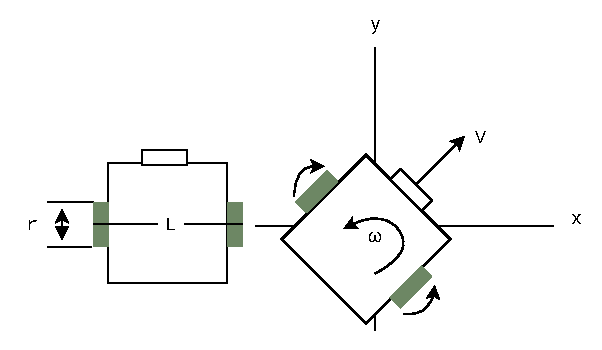
\includegraphics[width=0.5\textwidth]{figure/robot_model.pdf}
    \caption{2輪ロボットのモデル図}
    \label{fig:robot_model}
\end{figure}

\subsubsection{順運動学}
順運動学では,各車輪の角速度$\dot{\theta}_R$および$\dot{\theta}_L$から,ロボットの並進速度$v$,角速度$\omega$,および自己位置を算出する.自己位置の計算は,ロボットの進行方向と回転を考慮して行う.

ロボットの並進速度$v$と角速度$\omega$は,次式で表される.
\begin{equation}
    v = \frac{r}{2} (\dot{\theta}_R + \dot{\theta}_L)
    \label{eq:forward_v}
\end{equation}
\begin{equation}
    \omega = \frac{r}{L} (\dot{\theta}_R - \dot{\theta}_L)
    \label{eq:forward_omega}
\end{equation}

これに基づき,ロボットの自己位置$(x, y)$と向き$\theta$の時間変化を次のように表す.
\begin{equation}
    \dot{x} = v \cos \theta
    \label{eq:forward_x}
\end{equation}
\begin{equation}
    \dot{y} = v \sin \theta
    \label{eq:forward_y}
\end{equation}
\begin{equation}
    \dot{\theta} = \omega
    \label{eq:forward_theta}
\end{equation}

これらの微分方程式を離散化することで,時刻$t_k$における位置と向きを計算することができる.離散化した式は次のようになる.
\begin{equation}
    x_{k+1} = x_k + v_k \cos \theta_k \Delta t
    \label{eq:discrete_x}
\end{equation}
\begin{equation}
    y_{k+1} = y_k + v_k \sin \theta_k \Delta t
    \label{eq:discrete_y}
\end{equation}
\begin{equation}
    \theta_{k+1} = \theta_k + \omega_k \Delta t
    \label{eq:discrete_theta}
\end{equation}
ここで,$\Delta t$は計算ステップの時間間隔を示す.

順運動学を用いることで,各車輪の角速度を基にロボットの現在位置と進行方向をリアルタイムで更新することが可能である.

\subsubsection{逆運動学}
逆運動学では,ロボットの並進速度$v$と角速度$\omega$から,
車輪の角速度$\dot{\theta}_R$および$\dot{\theta}_L$を求める.
ロボットの基本的なモデルを図\ref{fig:robot_model}に示す.

ロボットの並進速度$v$および角速度$\omega$は,
車輪の角速度$\dot{\theta}_R$および$\dot{\theta}_L$により次式で表される.
\begin{equation}
    v = \frac{r}{2} (\dot{\theta}_R + \dot{\theta}_L)
    \label{eq:v}
\end{equation}
\begin{equation}
    \omega = \frac{r}{L} (\dot{\theta}_R - \dot{\theta}_L)
    \label{eq:omega}
\end{equation}

式\eqref{eq:v}および式\eqref{eq:omega}を連立すると,次のように導出できる.
\begin{equation}
    \dot{\theta}_R = \frac{1}{r} (v + \frac{L}{2} \omega)
    \label{eq:theta_R}
\end{equation}
\begin{equation}
    \dot{\theta}_L = \frac{1}{r} (v - \frac{L}{2} \omega)
    \label{eq:theta_L}
\end{equation}

これらの式により,目標速度$v$と$\omega$が与えられた場合に,
車輪の角速度$\dot{\theta}_R$と$\dot{\theta}_L$を算出し,
モータードライバを介して制御することでロボットの移動を実現できる.

\subsection{PID制御とローパスフィルタ}
PID制御(Proportional-Integral-Derivative Control)は,
制御工学における最も基本的かつ広く使用されているフィードバック制御の手法である.
本節では,PID制御の基本構造とローパスフィルタについて説明する.

\subsubsection{PID制御の構造}
PID制御は,目標値と現在値の偏差(エラー)を基に制御量を算出し,システムを目標値へ収束させる手法である.
制御量$u(t)$は次式で定義される:
\begin{equation}
    u(t) = K_P e(t) + K_I \int_{0}^{t} e(\tau) d\tau + K_D \frac{de(t)}{dt}
    \label{eq:pid}
\end{equation}
ここで,
\begin{itemize}
    \item $e(t)$:目標値と現在値の偏差
    \item $K_P$:比例ゲイン(P制御)
    \item $K_I$:積分ゲイン(I制御)
    \item $K_D$:微分ゲイン(D制御)
\end{itemize}
各項の役割は以下の通りである:
\begin{itemize}
    \item 比例制御(P制御):偏差に比例した制御量を生成し,応答の速さを向上させる.
    \item 積分制御(I制御):偏差を累積することで,定常偏差を排除する.
    \item 微分制御(D制御):偏差の変化率を基に,過渡応答の振動を抑制する.
\end{itemize}

\begin{figure}[h]
    \centering
    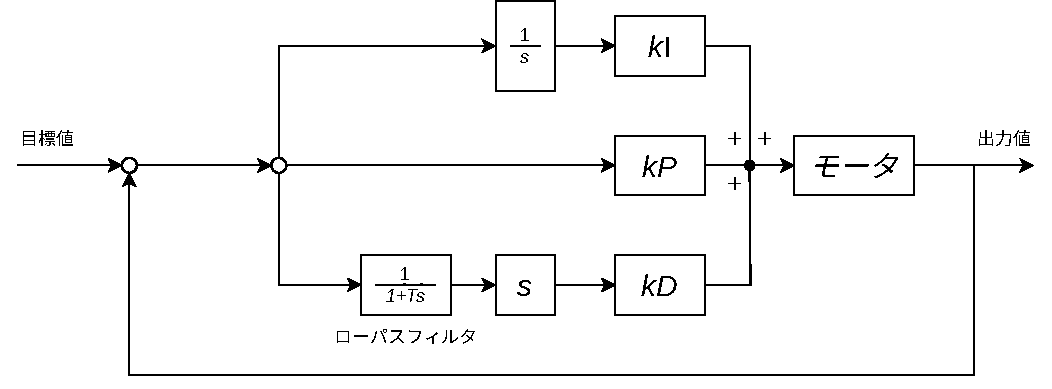
\includegraphics[width=0.7\textwidth]{figure/pid.pdf}
    \caption{PID制御器の構成図}
    \label{fig:pid_controller}
\end{figure}

図\ref{fig:pid_controller}にPID制御器の構成図を示す.
本研究では,このPID制御器を用いてロボットの速度を制御し,目標値への迅速かつ正確な追従を実現する.

\subsubsection{ローパスフィルタの導入}
微分制御(D制御)は高周波ノイズに敏感であり,そのまま使用するとシステムの安定性を損なう可能性がある.
この問題を軽減するために,微分項にローパスフィルタを適用することが一般的である.

ローパスフィルタを適用した微分制御項は次式で表される:
\begin{equation}
    D(s) = \frac{K_D s}{1 + T s}
    \label{eq:lowpass_filter}
\end{equation}
ここで,
\begin{itemize}
    \item $T$:ローパスフィルタの時定数
\end{itemize}

フィルタを導入することで,高周波ノイズが減衰され,システムの安定性が向上する.

\subsection{YOLOv5による物体認識}
本研究では,人の認識にYOLOv5(You Only Look Once Version 5)を使用する.
YOLOはリアルタイムで物体を検出するアルゴリズムであり,
1枚の画像に対して物体のクラスとその位置を同時に出力する特徴を持つ.
単一のニューラルネットワークを用いて,画像内の物体のバウンディングボックスとクラスラベルを直接予測する\cite{yolo}.
そのため他の物体検出モデル(例えばSSDやFaster R-CNN)と比較して,
高速な推論速度と高い精度を両立している.このため,リアルタイム性が要求されるロボットシステムにおいて有用である.

\subsubsection{人認識への応用}
本研究では,YOLOv5を用いてデプスカメラD435iから得られたRGB画像内の人を認識する.
YOLOv5は以下のステップで物体を検出する:
\begin{enumerate}
    \item RGB画像を入力し,YOLOv5のバックボーンにより特徴を抽出する.
    \item ネックでスケールを調整し,特徴を統合する.
    \item ヘッドでバウンディングボックス,クラスラベル(人),および信頼度スコアを出力する.
\end{enumerate}

出力されたバウンディングボックスは,ピクセル座標で記述されており,
これをデプスカメラのデプスマップと組み合わせることで,物理座標を算出する.
例えば,検出された人物のバウンディングボックス中心の座標$(u, v)$に対応するデプス値$Z$を用いて,
以下の式によりカメラ座標$(X_c, Y_c, Z_c)$を求める:
\begin{equation}
    X_c = \frac{(u - c_x) \cdot Z}{f_x}, \quad
    Y_c = \frac{(v - c_y) \cdot Z}{f_y}, \quad
    Z_c = Z
\end{equation}

この手法により,検出された人物の位置を3次元空間で特定することができる.


\subsection{デプスカメラと距離測定の方法}
デプスカメラは,対象物までの距離を計測するためのデバイスであり,ロボットの環境認識や障害物回避,
物体追跡などの応用において重要な役割を果たす.
本研究では,インテル® RealSense™ デプスカメラ D435iを使用し,
カメラから取得したデプスデータを基に人追従アルゴリズムを実現する.
本節では,デプスカメラの仕組みおよびD435iの特徴について説明する.

\subsubsection{デプスカメラの仕組み}
デプスカメラは,主に以下の3つの方式で距離を測定する:
\begin{itemize}
    \item ステレオカメラ方式:2つのカメラで撮影した画像から視差(パララックス)を計算し,
          物体までの距離を推定する.
    \item アクティブ赤外線方式:赤外線を投射し,反射光のパターンを解析することで深度情報を取得する.
    \item Time-of-Flight(ToF)方式:光の飛行時間を測定し,物体までの距離を直接計算する.
\end{itemize}

RealSense D435iは,ステレオカメラ方式を基本とし,アクティブ赤外線方式を補助的に使用する.
これにより,低照度環境やテクスチャの少ない物体に対しても安定した距離測定が可能となっている.

\subsection{デプスデータからの人座標検出}

\begin{figure}[h]
    \centering
    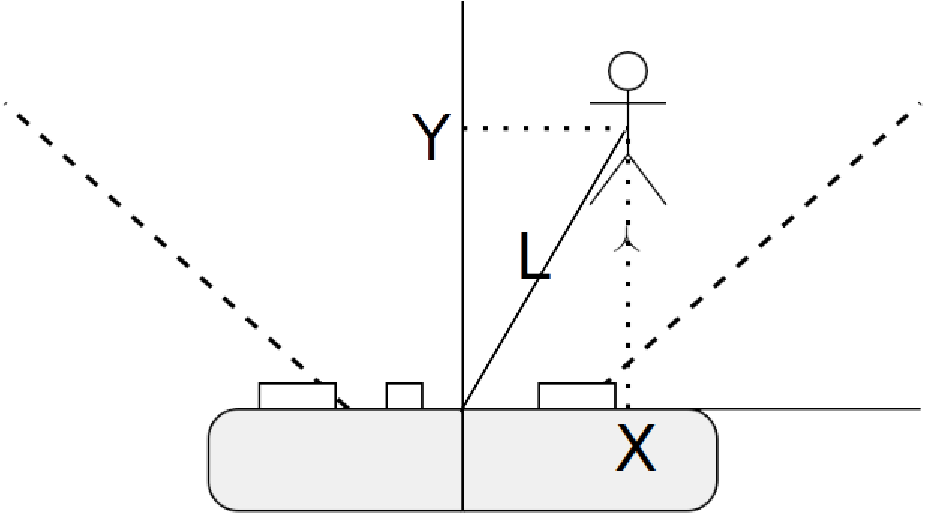
\includegraphics[width=0.4\textwidth]{figure/rialsens_man.pdf}
    \caption{デプスカメラを用いた座標変換モデル}
    \label{fig:coordinate_conversion}
\end{figure}

デプスカメラで取得したデータを用いて,画像上のピクセル座標を実空間の物理座標に変換することで,
人の位置を検出する.図\ref{fig:coordinate_conversion}に示すように,ピクセル座標系における対象物の位置を,
カメラ座標系に変換する手順を以下に述べる.

\subsubsection{ピクセル座標からカメラ座標への変換}
デプスカメラのデプスマップは,画像として各ピクセルの深度情報(距離)を格納している.このデータを利用して,ピクセル座標$(u, v)$をカメラ座標$(X_c, Y_c, Z_c)$に変換する.変換には以下の式を使用する:
\begin{equation}
    X_c = \frac{(u - c_x) \cdot Z_c}{f_x}
    \label{eq:xc}
\end{equation}
\begin{equation}
    Y_c = \frac{(v - c_y) \cdot Z_c}{f_y}
    \label{eq:yc}
\end{equation}
\begin{equation}
    Z_c = D(u, v)
    \label{eq:zc}
\end{equation}
ここで,
\begin{itemize}
    \item $u, v$:ピクセル座標系の位置 [pixel]
    \item $c_x, c_y$:カメラの光学中心 [pixel]
    \item $f_x, f_y$:カメラの焦点距離 [pixel]
    \item $D(u, v)$:デプスマップから取得される深度値 [m]
\end{itemize}

この変換により,画像上の対象物がカメラ座標系における3次元位置として表現される.

\subsubsection{カメラ座標からロボット座標への変換}
次に,カメラ座標$(X_c, Y_c, Z_c)$をロボット座標$(X_r, Y_r, Z_r)$に変換する.カメラとロボットの座標系の関係は,以下のように平行移動と回転を適用して記述される:
\begin{equation}
    \begin{bmatrix}
        X_r \\ Y_r \\ Z_r \\ 1
    \end{bmatrix}
    =
    \begin{bmatrix}
        R & T \\
        0 & 1
    \end{bmatrix}
    \begin{bmatrix}
        X_c \\ Y_c \\ Z_c \\ 1
    \end{bmatrix}
\end{equation}
ここで,
\begin{itemize}
    \item $R$:カメラ座標系からロボット座標系への回転行列
    \item $T$:カメラ座標系からロボット座標系への平行移動ベクトル
\end{itemize}

これにより,ロボット座標系において対象物の位置が求められる.

本研究では,D435iのデプスマップを利用して人の位置を検出し,ロボットの進行方向を計算する.
図\ref{fig:coordinate_conversion}に示すように,人の座標$(X_r, Y_r)$を基に追従アルゴリズムを適用し,
目標の移動方向を決定する.
 \newpage
% !TEX root = main.tex
\section{システム構成}
\subsection{システム全体図}
本研究で構築したシステムの全体図を図\ref{fig:system_diagram}に示す.
本システムは,下位レイヤーと上位レイヤーの2つの主要な構成要素からなる.

\begin{figure}[h]
    \centering
    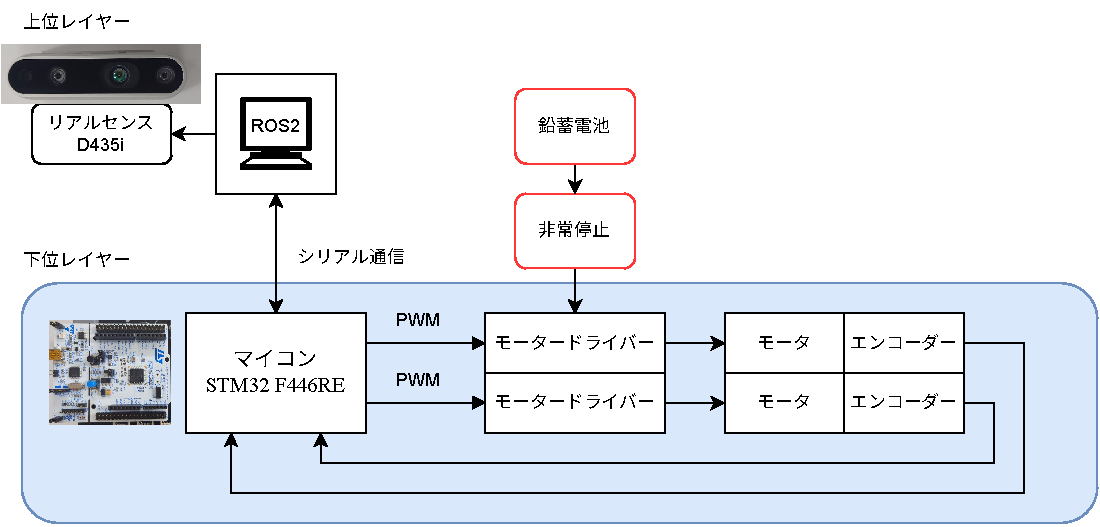
\includegraphics[width=1.0\textwidth]{figure/system.pdf}
    \caption{システム全体図}
    \label{fig:system_diagram}
\end{figure}

% === ハードウェア ==========================================================

\subsection{ハードウェア構成}
本システムのハードウェア構成について,以下に各要素を説明する.

\subsubsection{マイコン(STM32 Nucleo Board STM32F446RE)}
本システムでは,STM32 Nucleo Board STM32F446REマイコンボードを使用している.
STM32 F446REは高性能なARM Cortex-M4プロセッサを搭載しており,以下の特徴を持つ.
\begin{itemize}
    \item 最大180 MHzのクロック速度
    \item タイマーをエンコーダモードに設定可能
    \item 開発/評価ボードであり入手性が高い
\end{itemize}
本マイコンは,モーター駆動,エンコーダーのデータ取得を担当しており,
ロボットの下位制御レイヤーを実現している.


\subsubsection{エンコーダー(AMT102-V)}
AMT102-Vエンコーダーを採用し,モーターの回転角速度および回転位置を計測している.
図\ref{fig:AMT102}に使用するエンコーダーを示す.
このエンコーダーは最大分解能は2048 PPR(Pulse Per Revolution)であり,
非接触方式である.
エンコーダーからの信号はマイコンで処理され,
車輪の速度制御や自己位置推定に使用する.

\begin{figure}[H]
    \centering
    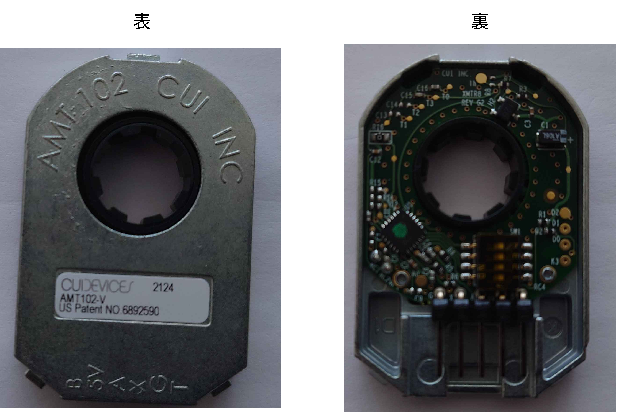
\includegraphics[width=0.5\textwidth]{figure/AMT102.pdf}
    \caption{AMT102-V}
    \label{fig:AMT102}
\end{figure}

\subsubsection{深度カメラ(Intel RealSense D435i)}
深度カメラとしてIntel RealSense D435iを採用している.D435iは,ステレオカメラ方式に基づく高精度な距離計測を特徴とし,以下のような仕様を持つ.
\begin{itemize}
    \item 最大測定距離:0.1~10メートル
    \item フレームレート:最大90 FPS
    \item 視野角:水平87°,垂直58°
    \item IMU(慣性計測ユニット)搭載
\end{itemize}
本システムでは,D435iから取得した深度データを用いて目標(人)の位置を検出し,
追従アルゴリズムに利用している.

\begin{figure}[H]
    \centering
    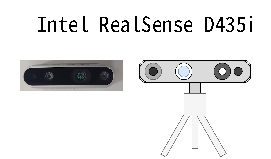
\includegraphics[width=0.5\textwidth]{figure/RealSense.pdf}
    \caption{AMT102-V}
    \label{fig:RealSense}
\end{figure}


% === ソフトウェア ==========================================================
\subsection{ソフトウェア構成}
本システムのソフトウェア構成について,以下に各要素を説明する.

\subsubsection{下位レイヤー}
本システムの下位レイヤーソフトウェアでは,モーター制御,エンコーダーのデータ処理,
およびシリアル通信を実現するために自作ライブラリを使用している.
以下に,各ライブラリの詳細について説明する.

\paragraph{エンコーダーライブラリ (encoder.c, encoder.h)}
エンコーダーライブラリは,ロータリーエンコーダー(AMT102-V)の値を取得し,
角速度や回転数を計算するための機能をもつ.
このライブラリでは,エンコーダーから得られる値を高精度に利用するために4逓倍処理を行い,
モーターの速度制御に使用している.以下に,一部ライブラリコードを示す.

\lstset{language=C}
\begin{figure}[H]
    \centering
    \begin{lstlisting}
int Encoder_Read(Encoder* encoder)
{
    int16_t count = (int16_t)(__HAL_TIM_GET_COUNTER(encoder->htim) - TIMER_MAX_COUNT / 2);
    return count;
}
        
void Encoder_Interrupt(Encoder* encoder, EncoderData* encoder_data)
{
    int count = Encoder_Read(encoder);
        
    encoder_data->count = count;
    encoder_data->rot = count / (double)encoder->ppr;
    encoder_data->deg = encoder_data->rot * 360.0;
    encoder_data->distance = encoder_data->rot * (PI * encoder->diameter);
        
    encoder_data->rps = (encoder_data->rot - encoder->before_rot) / (encoder->period * 0.001);
    encoder_data->velocity = encoder_data->rps * PI * encoder->diameter;
        
    encoder->before_rot = encoder_data->rot;
}
    \end{lstlisting}
    \caption{エンコーダーカウント値の取得 (encoder.c)}
    \label{lst:encoder_count}
\end{figure}

また,このライブラリではカウント値のリセット機能も提供しており,
特定の条件下でカウント値をゼロに戻すことが可能である.

\paragraph{モータードライバライブラリ (motor\_driver.c, motor\_driver.h)}
モータードライバライブラリは,DCモーターの速度と方向を制御するための機能をもつ.
このライブラリでは,PWM信号を用いてモーターを駆動し,
回転方向の切り替えや速度制御を行っていおる.以下に,一部ライブラリコードを示す.

\begin{figure}[H]
    \centering
    \begin{lstlisting}
// 初期化関数
void MotorDriver_Init(MotorDriver* motor, TIM_HandleTypeDef* htimA, uint32_t channelA,TIM_HandleTypeDef* htimB, uint32_t channelB) {
motor->htimA = htimA;
motor->channelA = channelA;
motor->htimB = htimB;
motor->channelB = channelB;    
 // PWM開始
HAL_TIM_PWM_Start(htimA, channelA);
HAL_TIM_PWM_Start(htimB, channelB);
}
// 速度設定関数
void MotorDriver_setSpeed(MotorDriver *motor, int speed) {
    int pwm_value;
    if (speed > 100) speed = 99;     //ブーストラップ回路に対応
    if (speed < -100) speed = -99;   //ブーストラップ回路に対応
        
    if (speed > 0) {
        pwm_value = (speed * __HAL_TIM_GET_AUTORELOAD(motor->htimA)) / 100;
        __HAL_TIM_SET_COMPARE(motor->htimA, motor->channelA, pwm_value);
        __HAL_TIM_SET_COMPARE(motor->htimB, motor->channelB, 0);
    } else {
        pwm_value = (-speed * __HAL_TIM_GET_AUTORELOAD(motor->htimA)) / 100;
        __HAL_TIM_SET_COMPARE(motor->htimA, motor->channelA, 0);
        __HAL_TIM_SET_COMPARE(motor->htimB, motor->channelB, pwm_value);
    }
}
    \end{lstlisting}
    \caption{モーターの速度設定 (motor\_driver.c)}
    \label{lst:motor_speed}
\end{figure}

\paragraph{シリアル通信ライブラリ (serial\_lib.c, serial\_lib.h)}
シリアル通信ライブラリは,PCや上位システムとのデータ通信を実現するために設計されている.
このライブラリでは,固定長および可変長データの送受信をサポートしており,
効率的かつ安全な通信を実現している.以下に,可変長データの送信および受信関数を示す.

この関数では,データを指定された形式に従ってパケット化し,
シリアル通信で送信する.
先頭にヘッダー(`SERIAL\_HEADER1` と `SERIAL\_HEADER2`)を追加し,
データ部分は16ビット整数をビッグエンディアン形式で格納する.
また,送信後に動的に確保したメモリを解放することで,メモリリークを防止している.

受信関数では,指定された形式に従って受信したデータをデコードし,
データバッファに格納する.受信データのヘッダーを検証し,
データが正しい形式であることを確認した後,各データを16ビット整数として復元する.
受信データが無効の場合,エラーコードを返すことで通信エラーを適切にハンドリングする.


\lstset{language=C}
\begin{figure}[H]
    \centering
    \begin{lstlisting}
// 可変長データの送信関数
void Serial_SendData(UART_HandleTypeDef *huart, int16_t *data, uint8_t data_count) {
    uint8_t buffer_size = 2 + data_count * 2;
    uint8_t *buffer = (uint8_t *)malloc(buffer_size);

    buffer[0] = SERIAL_HEADER1;
    buffer[1] = SERIAL_HEADER2;

    for (uint8_t i = 0; i < data_count; i++) {
        buffer[2 + i * 2] = (data[i] >> 8) & 0xFF;
        buffer[3 + i * 2] = data[i] & 0xFF;
    }

    HAL_UART_Transmit(huart, buffer, buffer_size, HAL_MAX_DELAY);
    free(buffer);
}
// 可変長データの受信関数
uint8_t Serial_ReceiveData(UART_HandleTypeDef *huart, int16_t *data, uint8_t data_count) {
    uint8_t buffer_size = 2 + data_count * 2;
    uint8_t *buffer = (uint8_t *)malloc(buffer_size);

    if (HAL_UART_Receive(huart, buffer, buffer_size, HAL_MAX_DELAY) == HAL_OK) {
        if (buffer[0] == SERIAL_HEADER1 && buffer[1] == SERIAL_HEADER2) {
            for (uint8_t i = 0; i < data_count; i++) {
                data[i] = (buffer[2 + i * 2] << 8) | buffer[3 + i * 2];
            }
            free(buffer);
            return 1; // 正常受信
        }
    }
    free(buffer);
    return 0; // エラー
}
    \end{lstlisting}
    \caption{可変長データの送受信関数 (serial\_lib.c)}
    \label{lst:serial}
\end{figure}


\paragraph{メインコード (main.c)}
メインコードでは,自作のエンコーダー,モータードライバ,シリアル通信ライブラリを統合し,
システム全体の制御を実現している.
このコードは,PCからの制御信号を受信してモーターの速度を設定するとともに,
エンコーダーから取得した速度データをPCに送信する役割を果たす.

この制御ループでは,まずシリアル通信ライブラリの`Serial\_ReceiveData`関数を使用して
PCからの制御信号を受信する.受信した制御信号は右車輪および左車輪の目標速度を表しており,
それぞれ`controlSignalRight`と`controlSignalLeft`に格納される.
これらの速度データは,モータードライバライブラリの`MotorDriver\_setSpeed`関数を用いて
設定される.

次に,エンコーダーデータの送信を行う.10msごとにタイマーの値を確認し,
タイミングが来た場合にエンコーダーライブラリの`Encoder\_Interrupt`関数を使用して
速度データを更新する.更新された速度データは,
シリアル通信ライブラリの`Serial\_SendData`関数を用いてPCに送信される.

このように,メインコードは上位システムとの通信,モーター制御,
およびエンコーダーデータの送信を連携させ,ロボット全体のリアルタイム制御を実現している.


以下に,一部実装コードを示す.

\lstset{language=C}
\begin{figure}[H]
    \centering
    \begin{lstlisting}
// メイン制御ループ
while (1)
{
    /* PCからの制御信号を受信 */
    int16_t receivedData[2];
    if (Serial_ReceiveData(&huart2, receivedData, 2))
    {
        controlSignalRight = receivedData[0];
        controlSignalLeft = receivedData[1];

        MotorDriver_setSpeed(&motorRight, -1 * controlSignalRight);
        MotorDriver_setSpeed(&motorLeft, -1 * controlSignalLeft);
    }

    /* エンコーダーデータの送信(10msごとに送信) */
    if (HAL_GetTick() - lastSendTime >= 10)
    {
        lastSendTime = HAL_GetTick();

        /* エンコーダーの速度データを更新 */
        Encoder_Interrupt(&encoderRight, &encoderDataRight);
        Encoder_Interrupt(&encoderLeft, &encoderDataLeft);

        /* エンコーダー速度を送信 */
        int16_t feedbackData[2] = {(int16_t)encoderDataRight.velocity, (int16_t)encoderDataLeft.velocity};
        Serial_SendData(&huart2, feedbackData, 2);
    }
}
    \end{lstlisting}
    \caption{メイン制御ループ (main.c)}
    \label{lst:main_loop}
\end{figure}

% !TEX root = main.tex
% === ハードウェア ==========================================================

\subsection{ハードウェア構成}
本システムのハードウェア構成について,以下に各要素を説明する.

\subsubsection{マイコン(STM32 Nucleo Board STM32F446RE)}
本システムでは,STM32 Nucleo Board STM32F446REマイコンボードを使用している.
STM32 F446REは高性能なARM Cortex-M4プロセッサを搭載しており,以下の特徴を持つ\cite{stm}.
\begin{itemize}
  \item ST-LINKデバッガ / プログラマが内蔵
  \item タイマーをエンコーダモードに設定可能
  \item 開発/評価ボードであり入手性が高い
\end{itemize}
本マイコンは,モーター駆動,エンコーダーのデータ取得を担当しており,
ロボットの下位制御レイヤーを実現している.


\subsubsection{エンコーダー(AMT102-V)}
AMT102-Vエンコーダーを採用し,モーターの回転角速度および回転位置を計測している.
図\ref{fig:AMT102}に使用するエンコーダーを示す.
このエンコーダーは最大分解能は5120 PPR(Pulse Per Revolution)であり,
非接触方式である\cite{amt}.
エンコーダーからの信号はマイコンで処理され,
車輪の速度制御やオドメトリに使用する.

\begin{figure}[H]
  \centering
  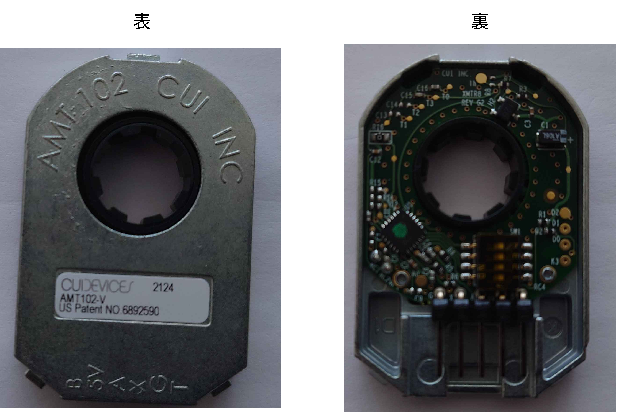
\includegraphics[width=0.4\textwidth]{figure/AMT102.pdf}
  \caption{AMT102-V}
  \label{fig:AMT102}
\end{figure}

\subsubsection{深度カメラ(Intel RealSense D435i)}
深度カメラとしてIntel RealSense D435iを採用している.
D435iは,ステレオカメラ方式に基づく高精度な距離計測を特徴とし,以下のような仕様を持つ\cite{realsense}.
\begin{itemize}
  \item 最大測定距離:0.1~10メートル
  \item 出力解像度(DepthStream):最大1280 x 720
  \item 出力フレームレート(DepthStream):最大90 fps
  \item RGB解像度およびフレームレート:1920 x 1080@30 fps
  \item 深度センサ視野角:水平85.2°,垂直58°
  \item IMU(慣性計測ユニット)搭載
\end{itemize}
本システムでは,D435iから取得した深度データを用いて目標(人)の位置を検出し,
追従アルゴリズムに利用している.

\begin{figure}[H]
  \centering
  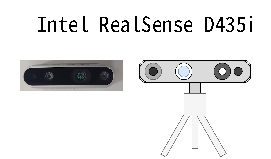
\includegraphics[width=0.5\textwidth]{figure/RealSense.pdf}
  \caption{RealSense}
  \label{fig:RealSense}
\end{figure}

D435iの内部パラメータ(焦点距離と光学中心)は,以下のPythonコードを使用して計測した.

\begin{lstlisting}[language=Python, caption=RealSense内部パラメータの取得]
import pyrealsense2 as rs

# RealSense パイプラインのセットアップ
pipeline = rs.pipeline()
config = rs.config()
config.enable_stream(rs.stream.depth, 640, 480, rs.format.z16, 30)
pipeline.start(config)

# 深度ストリームのプロファイルからカメラパラメータを取得
profile = pipeline.get_active_profile()
depth_stream = profile.get_stream(rs.stream.depth)  # 深度ストリーム
intrinsics = depth_stream.as_video_stream_profile().get_intrinsics()

# 内部パラメータを取得
fx = intrinsics.fx  # 焦点距離 (f_x)
fy = intrinsics.fy  # 焦点距離 (f_y)
cx = intrinsics.ppx  # 光学中心 x 座標 (c_x)
cy = intrinsics.ppy  # 光学中心 y 座標 (c_y)

print(f"焦点距離: fx={fx}, fy={fy}")
print(f"光学中心: cx={cx}, cy={cy}")

# 使用後はパイプラインを停止
pipeline.stop()
\end{lstlisting}

このコードを実行した結果,D435iの焦点距離と光学中心が以下の通り得られた.

\begin{itemize}
  \item 焦点距離:$f_x = 378.09$ [pixel],$f_y = 378.09$ [pixel]
  \item 光学中心:$c_x = 319.39$ [pixel],$c_y = 237.10$ [pixel]
\end{itemize}

これらの内部パラメータは,ピクセル座標系からカメラ座標系への変換(式\eqref{eq:xc},\eqref{eq:yc})で使用される.
% !TEX root = main.tex

% === ソフトウェア ==========================================================
\subsection{ソフトウェア構成}
本システムのソフトウェア構成について,以下に各要素を説明する.


% === 下位レイヤー ==========================================================
\subsubsection{下位レイヤー}
本システムの下位レイヤーソフトウェアでは,モーター制御,エンコーダーのデータ処理,
およびシリアル通信を実現するために自作ライブラリを使用している.
開発環境はCubeIED(ver.1.16.1)である.
以下に,各ライブラリの詳細について説明する.

\paragraph{エンコーダーライブラリ (encoder.c, encoder.h)}\mbox{}\\
エンコーダーライブラリは,ロータリーエンコーダー(AMT102-V)の値を取得し,
角速度や回転数を計算するための機能をもつ.
このライブラリでは,エンコーダーから得られる値を高精度に利用するために4逓倍処理を行い,
モーターの速度制御に使用している.以下に,一部ライブラリコードを示す.


\lstset{language=C, caption={エンコーダーカウント値の取得}}

\begin{lstlisting}
    // エンコーダーカウント値の取得
    int Encoder_Read(Encoder* encoder)
    {
        int16_t count = (int16_t)(__HAL_TIM_GET_COUNTER(encoder->htim) - TIMER_MAX_COUNT / 2);
        return count;
    }
    
    void Encoder_Interrupt(Encoder* encoder, EncoderData* encoder_data)
    {
        int count = Encoder_Read(encoder);
    
        encoder_data->count = count;
        encoder_data->rot = count / (double)encoder->ppr;
        encoder_data->deg = encoder_data->rot * 360.0;
        encoder_data->distance = encoder_data->rot * (PI * encoder->diameter);
    
        encoder_data->rps = (encoder_data->rot - encoder->before_rot) / (encoder->period * 0.001);
        encoder_data->velocity = encoder_data->rps * PI * encoder->diameter;
    
        encoder->before_rot = encoder_data->rot;
    }
\end{lstlisting}

また,このライブラリではカウント値のリセット機能も提供しており,
特定の条件下でカウント値をゼロに戻すことが可能である.

\paragraph{モータードライバライブラリ (motor\_driver.c, motor\_driver.h)}\mbox{}\\
モータードライバライブラリは,DCモーターの速度と方向を制御するための機能をもつ.
このライブラリでは,PWM信号を用いてモーターを駆動し,
回転方向の切り替えや速度制御を行っていおる.
以下に,一部ライブラリコードを示す.

\lstset{language=C, caption=モーターの速度設定 (motor\_driver.c)}

\begin{lstlisting}
// 初期化関数
void MotorDriver_Init(MotorDriver* motor, TIM_HandleTypeDef* htimA, uint32_t channelA,TIM_HandleTypeDef* htimB, uint32_t channelB) {
motor->htimA = htimA;
motor->channelA = channelA;
motor->htimB = htimB;
motor->channelB = channelB;    
 // PWM 開始
HAL_TIM_PWM_Start(htimA, channelA);
HAL_TIM_PWM_Start(htimB, channelB);
}
// 速度設定関数
void MotorDriver_setSpeed(MotorDriver *motor, int speed) {
    int pwm_value;
    if (speed > 100) speed = 99;     //ブーストラップ回路に対応
    if (speed < -100) speed = -99;   //ブーストラップ回路に対応
        
    if (speed > 0) {
        pwm_value = (speed * __HAL_TIM_GET_AUTORELOAD(motor->htimA)) / 100;
        __HAL_TIM_SET_COMPARE(motor->htimA, motor->channelA, pwm_value);
        __HAL_TIM_SET_COMPARE(motor->htimB, motor->channelB, 0);
    } else {
        pwm_value = (-speed * __HAL_TIM_GET_AUTORELOAD(motor->htimA)) / 100;
        __HAL_TIM_SET_COMPARE(motor->htimA, motor->channelA, 0);
        __HAL_TIM_SET_COMPARE(motor->htimB, motor->channelB, pwm_value);
    }
}
\end{lstlisting}


\paragraph{シリアル通信ライブラリ (serial\_lib.c, serial\_lib.h)}\mbox{}\\
シリアル通信ライブラリは,PCや上位システムとのデータ通信を実現するために設計されている.
このライブラリでは,固定長および可変長データの送受信をサポートしており,
効率的かつ安全な通信を実現している.以下に,可変長データの送信および受信関数を示す.

\lstset{language=C, caption=可変長データの送受信関数 (serial\_lib.c)}

\begin{lstlisting}
// 可変長データの送信関数
void Serial_SendData(UART_HandleTypeDef *huart, int16_t *data, uint8_t data_count) {
    uint8_t buffer_size = 2 + data_count * 2;
    uint8_t *buffer = (uint8_t *)malloc(buffer_size);

    buffer[0] = SERIAL_HEADER1;
    buffer[1] = SERIAL_HEADER2;

    for (uint8_t i = 0; i < data_count; i++) {
        buffer[2 + i * 2] = (data[i] >> 8) & 0xFF;
        buffer[3 + i * 2] = data[i] & 0xFF;
    }

    HAL_UART_Transmit(huart, buffer, buffer_size, HAL_MAX_DELAY);
    free(buffer);
}
// 可変長データの受信関数
uint8_t Serial_ReceiveData(UART_HandleTypeDef *huart, int16_t *data, uint8_t data_count) {
    uint8_t buffer_size = 2 + data_count * 2;
    uint8_t *buffer = (uint8_t *)malloc(buffer_size);

    if (HAL_UART_Receive(huart, buffer, buffer_size, HAL_MAX_DELAY) == HAL_OK) {
        if (buffer[0] == SERIAL_HEADER1 && buffer[1] == SERIAL_HEADER2) {
            for (uint8_t i = 0; i < data_count; i++) {
                data[i] = (buffer[2 + i * 2] << 8) | buffer[3 + i * 2];
            }
            free(buffer);
            return 1; // 正常受信
        }
    }
    free(buffer);
    return 0; // エラー
}
\end{lstlisting}

この関数では,データを指定された形式に従ってパケット化し,
シリアル通信で送信する.
先頭にヘッダー(`SERIAL\_HEADER1` と `SERIAL\_HEADER2`)を追加し,
データ部分は16ビット整数をビッグエンディアン形式で格納する.
また,送信後に動的に確保したメモリを解放することで,メモリリークを防止している.

受信関数では,指定された形式に従って受信したデータをデコードし,
データバッファに格納する.受信データのヘッダーを検証し,
データが正しい形式であることを確認した後,各データを16ビット整数として復元する.
受信データが無効の場合,エラーコードを返すことで通信エラーを適切にハンドリングする.


\paragraph{メインコード (main.c)}\mbox{}\\
メインコードでは,自作のエンコーダー,モータードライバ,シリアル通信ライブラリを統合し,
システム全体の制御を実現している.
このコードは,PCからの制御信号を受信してモーターの速度を設定するとともに,
エンコーダーから取得した速度データをPCに送信する役割を果たす.

この制御ループでは,まずシリアル通信ライブラリの`Serial\_ReceiveData`関数を使用して
PCからの制御信号を受信する.受信した制御信号は右車輪および左車輪の目標速度を表しており,
それぞれ`controlSignalRight`と`controlSignalLeft`に格納される.
これらの速度データは,モータードライバライブラリの`MotorDriver\_setSpeed`関数を用いて
設定される.

次に,エンコーダーデータの送信を行う.10msごとにタイマーの値を確認し,
タイミングが来た場合にエンコーダーライブラリの`Encoder\_Interrupt`関数を使用して
速度データを更新する.更新された速度データは,
シリアル通信ライブラリの`Serial\_SendData`関数を用いてPCに送信される.

このように,メインコードは上位システムとの通信,モーター制御,
およびエンコーダーデータの送信を連携させ,ロボット全体のリアルタイム制御を実現している.


以下に,一部実装コードを示す.

\lstset{language=C, caption=メイン制御ループ (main.c)}
\begin{lstlisting}
// メイン制御ループ
while (1)
{
    /* PC からの制御信号を受信 */
    int16_t receivedData[2];
    if (Serial_ReceiveData(&huart2, receivedData, 2))
    {
        controlSignalRight = receivedData[0];
        controlSignalLeft = receivedData[1];

        MotorDriver_setSpeed(&motorRight, -1 * controlSignalRight);
        MotorDriver_setSpeed(&motorLeft, -1 * controlSignalLeft);
    }

    /* エンコーダーデータの送信( 10[ms] ごとに送信) */
    if (HAL_GetTick() - lastSendTime >= 10)
    {
        lastSendTime = HAL_GetTick();

        /* エンコーダーの速度データを更新 */
        Encoder_Interrupt(&encoderRight, &encoderDataRight);
        Encoder_Interrupt(&encoderLeft, &encoderDataLeft);

        /* エンコーダー速度を送信 */
        int16_t feedbackData[2] = {(int16_t)encoderDataRight.velocity, (int16_t)encoderDataLeft.velocity};
        Serial_SendData(&huart2, feedbackData, 2);
    }
}
\end{lstlisting}


% === 上位レイヤー ==========================================================
\subsubsection{上位レイヤー}
本システムの上位レイヤーでは,以下のROS2ノードを利用してリアルタイムなデータ処理と通信を実現している.
開発環境はROS2 humble ,Python 3.10.12 である.

本研究で使用したROS2ノードは以下の通りである.
\begin{itemize}
    \item \textbf{web\_socket\_node}: Webブラウザと通信し,ロボットに指令を与える.
    \item \textbf{PID\_node}: PID制御を用いてモーター制御信号を生成.
    \item \textbf{RealSense\_node}: 深度カメラからデータを取得し,ターゲットの位置を推定.
    \item \textbf{serial\_read\_node}: 下位レイヤーとのシリアル通信を通じてエンコーダーデータを受信.
    \item \textbf{serial\_send\_node}: モーター制御信号を下位レイヤーに送信.
    \item \textbf{Roboware\_node}: ロボット全体の管理,および追従アルゴリズムを搭載.
\end{itemize}

図\ref{fig:rqt}にrqt\_graphによりノード間の接続状況を視覚化したものを示す.

\begin{figure}[H]
    \centering
    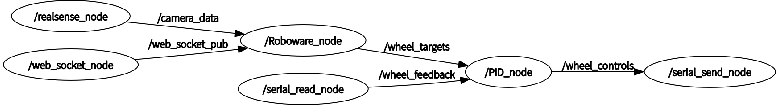
\includegraphics[width=1.0\textwidth]{figure/rqtgraph_v1.4.pdf}
    \caption{rqtgraph}
    \label{fig:rqt}
\end{figure}


\paragraph{web\_socket\_node}\mbox{}\\
web\_socket\_nodeは,FastAPIを使用してWebブラウザとROS2ノード間の双方向通信を行う.
Webブラウザからはロボットの制御指令を送信でき,ロボットの現在位置や状態をリアルタイムで取得できる.

FastAPIは軽量かつ高性能なWebフレームワークであり,非同期通信をサポートするため,
WebSocketを用いたリアルタイム通信にも対応している.
WebSocketは、HTTPプロトコルを拡張した双方向通信のためのプロトコルであり,効率的なデータ送受信を可能にする.

\begin{itemize}
    \item \textbf{購読トピック}
          \begin{itemize}
              \item \texttt{estimated\_position} (\texttt{Float32MultiArray}): 推定位置データ
          \end{itemize}
    \item \textbf{発行トピック}
          \begin{itemize}
              \item \texttt{web\_socket\_pub} (\texttt{String}): WebSocket通信で受信したコマンド
          \end{itemize}
\end{itemize}


以下に,WebSocket通信の主要な実装部分を示す.

\begin{lstlisting}[language=Python, caption=WebSocket通信の主要部分 (web\_socket\_node.py)]
# FastAPI インスタンスの作成
app = FastAPI()

# WebSocket 通信のエンドポイント
@app.websocket('/ws')
async def websocket_endpoint(websocket: FastAPIWebSocket):
    await websocket.accept()
    try:
        while True:
            # クライアントからのデータを受信
            receive_data = await websocket.receive_text()
            
            # ROS トピックにデータをパブリッシュ
            msg = String()
            msg.data = receive_data
            self.pub.publish(msg)

            # サブスクライブしたデータをクライアントに送信
            string_send_data = ",".join(map(str, self.send_data))
            await websocket.send_text(string_send_data)
    except Exception as e:
        print(f'WebSocket error: {str(e)}')
    finally:
        print('WebSocket disconnected')
\end{lstlisting}

この実装では,Webブラウザから送信された制御信号をROSトピック`web\_socket\_pub`にパブリッシュし,
ROS2ノードで処理される.
同時に,ROS2ノードがサブスクライブしたデータをWebブラウザに送信することでリアルタイム通信を実現している.


\paragraph{PID\_node}\mbox{}\\
PID\_nodeは,ロボットのモーター制御信号を生成するためにPID制御アルゴリズムを実装したノードである.
PID制御では,目標値と現在値の差(偏差)を基に比例(P),積分(I),微分(D)の3要素を組み合わせて制御信号を生成する.
さらに,本ノードでは微分項にローパスフィルタを適用し,ノイズの影響を低減している.

本ノードは以下のROSトピックを使用する.
\begin{itemize}
    \item \textbf{購読トピック}
          \begin{itemize}
              \item \texttt{wheel\_targets} (\texttt{Float32MultiArray}): 目標速度データ(右車輪,左車輪)
              \item \texttt{wheel\_feedback} (\texttt{Float32MultiArray}): 現在速度データ(右車輪,左車輪)
          \end{itemize}
    \item \textbf{発行トピック}
          \begin{itemize}
              \item \texttt{wheel\_controls} (\texttt{Float32MultiArray}): 制御信号(右車輪,左車輪)
          \end{itemize}
\end{itemize}

以下に,PID制御アルゴリズムの主要な実装部分を示す.

\begin{lstlisting}[language=Python, caption=PID制御アルゴリズムの実装 (PID\_node.py)]
class PIDController:
    def __init__(self, kp, ki, kd, tau=0.01):
        self.kp = kp
        self.ki = ki
        self.kd = kd
        self.tau = tau  # ローパスフィルタの時定数
        self.prev_error = 0.0
        self.integral = 0.0
        self.prev_derivative = 0.0  # 前回の微分値

    def compute(self, target, current, dt):
        error = target - current
        self.integral += error * dt

        # 微分項にローパスフィルタを適用
        raw_derivative = (error - self.prev_error) / dt
        derivative = (self.tau * self.prev_derivative + dt * raw_derivative) / (self.tau + dt)
        self.prev_derivative = derivative
        self.prev_error = error

        return self.kp * error + self.ki * self.integral + self.kd * derivative
\end{lstlisting}

このアルゴリズムでは,目標速度と現在速度の差を計算し,PID制御の各要素を基に制御信号を生成する.
ローパスフィルタを導入することで,ノイズによる微分項の影響を抑制し,安定した制御信号を生成する.

次に,制御ループの主要部分を以下に示す.

\begin{lstlisting}[language=Python, caption=制御ループ (PID\_node.py)]
def control_loop(self):
    current_time = self.get_clock().now()
    dt = (current_time - self.last_time).nanoseconds / 1e9
    self.last_time = current_time

    # 右車輪と左車輪の制御信号を計算
    control_signal_right = self.pid_right.compute(self.target_right, self.current_right, dt)
    control_signal_left = self.pid_left.compute(self.target_left, self.current_left, dt)

    # 制御信号をパブリッシュ
    control_msg = Float32MultiArray()
    control_msg.data = [float(control_signal_right), float(control_signal_left)]
    self.pub.publish(control_msg)
\end{lstlisting}

この制御ループでは,以下の手順でモーター制御信号を生成する.
\begin{enumerate}
    \item 目標速度と現在速度の偏差を計算し,PID制御を実行.
    \item 生成した制御信号をROSトピック\texttt{wheel\_controls}にパブリッシュ.
    \item デバッグ用に制御信号の詳細をログ出力.
\end{enumerate}

これにより,ロボットの速度を目標値に追従させるためのリアルタイム制御が可能となる.


\paragraph{RealSense\_node}\mbox{}\\
RealSense\_nodeは,Intel RealSense D435iカメラを使用して深度データとRGB画像を処理し,ターゲットの検出および距離・オフセット情報を生成する.このノードは,YOLOv5を利用した物体検出アルゴリズムを実装しており,人物の位置と距離をリアルタイムで推定してパブリッシュする.

本ノードは以下のROSトピックを使用する.
\begin{itemize}
    \item \textbf{発行トピック}
          \begin{itemize}
              \item \texttt{camera\_data} (\texttt{Float32MultiArray}): 人物の距離とオフセット情報
          \end{itemize}
\end{itemize}

以下に,主要な処理と実装部分を示す.

\begin{lstlisting}[language=Python, caption=ターゲット検出と距離推定 (RealSense\_node.py)]
# RealSense フレームの処理
def process_frames(self):
    try:
        frames = self.pipeline.wait_for_frames()
        depth_frame = frames.get_depth_frame()
        color_frame = frames.get_color_frame()
        if not depth_frame or not color_frame:
            return

        # 深度データとRGB データを取得
        depth_image = np.asanyarray(depth_frame.get_data())
        color_image = np.asanyarray(color_frame.get_data())

        # YOLOv5 による物体検出
        results = self.model(color_image)
        for result in results.xyxy[0]:  # 検出結果をループ
            box, conf, cls = result[:4], result[4], int(result[5])
            if cls == 0:  # クラス0(人物)のみ処理
                x1, y1, x2, y2 = map(int, box)
                center_x, center_y = (x1 + x2) // 2, (y1 + y2) // 2

                # 深度データから距離とオフセットを計算
                raw_distance = depth_frame.get_distance(center_x, center_y)
                offset_x = center_x - (color_image.shape[1] // 2)
                filtered_distance = self.filter_distance(raw_distance)

                # データをパブリッシュ
                msg = Float32MultiArray()
                msg.data = [filtered_distance, float(offset_x)]
                self.publisher.publish(msg)

                # デバッグ情報の表示
                self.get_logger().info(
                    f"Published camera data: Distance={filtered_distance:.2f}, Offset={offset_x}"
                )
                break
    except Exception as e:
        self.get_logger().error(f"Error processing frames: {str(e)}")
\end{lstlisting}

距離データは,近づく場合はそのままの値を使用し,遠ざかる場合は移動平均フィルタを適用している.
このフィルタリングは,測定誤差やノイズの影響を低減するためである.

\begin{lstlisting}[language=Python, caption=距離データのフィルタリング (RealSense\_node.py)]
def filter_distance(self, current_distance):
    if current_distance == 0.0:  # 無効値は無視
        return self.previous_distance

    if current_distance < self.previous_distance:
        # 近づいている場合: そのままの値を使用
        self.distance_history = [current_distance]  # 履歴をリセット
        return current_distance
    else:
        # 遠ざかる場合: 移動平均フィルタを適用
        self.distance_history.append(current_distance)
        if len(self.distance_history) > self.history_size:
            self.distance_history.pop(0)  # 古い値を削除
        return sum(self.distance_history) / len(self.distance_history)
\end{lstlisting}

本ノードは,RealSenseカメラから取得した深度データとRGB画像をもとに,
YOLOv5を用いたターゲット検出と距離推定を行い,リアルタイムでROSトピックに結果をパブリッシュする.

\paragraph{serial\_read\_node}\mbox{}\\
serial\_read\_nodeは,下位レイヤーから送信されるエンコーダーデータをシリアル通信を通じて受信し,
ROSトピックにパブリッシュする役割を持つ.
このノードは非同期通信をサポートしており,リアルタイムでのデータ受信とパブリッシュを実現している.

\begin{itemize}
    \item \textbf{発行トピック}
          \begin{itemize}
              \item \texttt{wheel\_feedback} (\texttt{Float32MultiArray}): エンコーダーデータ(右車輪,左車輪)
          \end{itemize}
\end{itemize}

以下に,主要なコード部分を示す.

\begin{lstlisting}[language=Python, caption=シリアルデータの受信とトピックへのパブリッシュ (serial\_read\_node.py)]
class SerialReadNode(Node):
    def __init__(self):
        super().__init__('serial_read_node')
        self.publisher = self.create_publisher(Float32MultiArray, 'wheel_feedback', 10)
        # シリアル通信の設定
        self.serial_port = serial.Serial('/dev/ttyUSB0', 115200, timeout=1)
        self.create_timer(0.1, self.read_serial_data)
    def read_serial_data(self):
        try:
            if self.serial_port.in_waiting > 0:
                data = self.serial_port.read(8)  # 8バイトを読み取る
                right_speed, left_speed = struct.unpack('>hh', data[2:])  # データのデコード
                msg = Float32MultiArray()
                msg.data = [float(right_speed), float(left_speed)]
                self.publisher.publish(msg)
                self.get_logger().info(f"Published wheel_feedback: {msg.data}")
        except Exception as e:
            self.get_logger().error(f"Error reading serial data: {str(e)}")
\end{lstlisting}

このノードでは,シリアルポートから受信したエンコーダーデータを解析し,
右車輪と左車輪の速度データとしてトピック\texttt{wheel\_feedback}にパブリッシュする.

\paragraph{serial\_send\_node}\mbox{}\\
serial\_send\_nodeは,上位レイヤーからのモーター制御信号を下位レイヤーに送信する役割を持つ.
このノードは,ROSトピックから制御信号を受け取り,指定されたフォーマットで
パケット化してシリアル通信を通じて下位レイヤーに送信する.

\begin{itemize}
    \item \textbf{購読トピック}
          \begin{itemize}
              \item \texttt{wheel\_controls} (\texttt{Float32MultiArray}): モーター制御信号(右車輪,左車輪)
          \end{itemize}
\end{itemize}

以下に,主要なコード部分を示す.

\begin{lstlisting}[language=Python, caption=制御信号の送信 (serial\_send\_node.py)]
class SerialSendNode(Node):
    def __init__(self):
        super().__init__('serial_send_node')
        self.subscription = self.create_subscription(
            Float32MultiArray,
            'wheel_controls',
            self.send_serial_data,
            10
        )
        # シリアル通信の設定
        self.serial_port = serial.Serial('/dev/ttyUSB0', 115200, timeout=1)
    def send_serial_data(self, msg):
        try:
            if len(msg.data) == 2:
                right_control, left_control = int(msg.data[0]), int(msg.data[1])
                data = struct.pack('>BBhh', 0xA5, 0xA5, right_control, left_control)
                self.serial_port.write(data)
                self.get_logger().info(f"Sent wheel_controls: {msg.data}")
        except Exception as e:
            self.get_logger().error(f"Error sending serial data: {str(e)}")
\end{lstlisting}

このノードでは,モーター制御信号をROSトピック\texttt{wheel\_controls}から受信し,
指定されたフォーマットでパケット化してシリアル通信を通じて送信する.


\paragraph{Roboware\_node}\mbox{}\\
Roboware\_nodeは,ロボットの速度制御を実現するためのノードであり,
比例航法 (PN),修正比例航法 (MPN),およびゲインスケジューリング下修正比例航法 (GS-MPN)
をサポートしている.
これらのアルゴリズムを用いて,ターゲットを追従する速度と角速度を計算し,
逆運動学を用いて車輪ごとの目標速度を決定する.

\begin{itemize}
    \item \textbf{購読トピック}
          \begin{itemize}
              \item \texttt{web\_socket\_pub} (\texttt{String}): 操作モードおよびロボット制御信号
              \item \texttt{camera\_data} (\texttt{Float32MultiArray}): 距離とオフセットデータ
          \end{itemize}
    \item \textbf{発行トピック}
          \begin{itemize}
              \item \texttt{wheel\_targets} (\texttt{Float32MultiArray}): 車輪ごとの目標速度
          \end{itemize}
\end{itemize}

以下に,各アルゴリズムでの速度計算部分を示す.

\subparagraph{PN (Proportional Navigation)}\mbox{}\\
PNアルゴリズムでは,以下のように直進速度$V$と角速度$\omega$を計算する.
\begin{lstlisting}[language=Python, caption=PNの計算部分 (Roboware\_node\_np.py)]
V = self.kp_v * (self.person_distance - 1.0)
omega = (self.navigation_constant) * self.kp_omega * self.person_offset / max((self.person_distance), 1.0)
\end{lstlisting}

\subparagraph{MPN (Modified Proportional Navigation)}\mbox{}\\
MPNでは,偏差角速度の微分を用いて動作をなめらかにするため,以下のように計算する.
\begin{lstlisting}[language=Python, caption=MPNの計算部分 (Roboware\_node\_mpn.py)]
offset_rate = (self.person_offset - self.previous_offset) / self.dt  # 偏差角速度
V = self.kp_v * (self.person_distance - 1.0)
omega = (
    self.navigation_constant * self.kp_omega * self.person_offset / self.person_distance +
    self.lambda_gain * offset_rate
)
self.previous_offset = self.person_offset  # 偏差を更新
\end{lstlisting}

\subparagraph{GS-MPN (Gain-Scheduled Modified Proportional Navigation)}\mbox{}\\
GS-MPNでは,動的微分ゲインを導入し,偏差角速度に基づく調整を行う.
\begin{lstlisting}[language=Python, caption=GS-MPNの計算部分 (Roboware\_node\_newmpn.py)]
offset_rate = (self.person_offset - self.previous_offset) / self.dt  # 偏差角速度
dynamic_kd = self.kd_lambda * (1 - math.exp(-self.a * abs(offset_rate))) / (1 + math.exp(-self.a * abs(offset_rate)))
V = self.kp_v * (self.person_distance - 1.0)
omega = (
    self.navigation_constant * self.kp_omega * self.person_offset / self.person_distance +
    dynamic_kd * offset_rate
)
self.previous_offset = self.person_offset  # 偏差を更新
\end{lstlisting}



計算された直進速度$V$と角速度$\omega$から,逆運動学を用いて右車輪および左車輪の速度を以下のように計算する.
\begin{lstlisting}[language=Python, caption=逆運動学を用いた車輪速度の計算]
self.target_right = (2 * V + omega * self.L) / (2 * self.r)
self.target_left = (2 * V - omega * self.L) / (2 * self.r)
\end{lstlisting}

また,カメラからの座標変換も行っている.
\begin{lstlisting}[language=Python, caption=座標変換]
def position_callback(self, msg):
    if len(msg.data) == 2:  
        pixel_offset = msg.data[1]  # カメラ画像上の水平ズレ(ピクセル)
        depth = msg.data[0]  # カメラから取得した深度値( m )
        # 座標変換
        x_camera = (pixel_offset * depth) / self.fx  # カメラ座標系のX
        y_camera = depth  # カメラ座標系のY

        # ロボット座標系への変換
        x_robot = x_camera + self.camera_offset_x
        y_robot = y_camera

        # 更新
        self.person_offset = x_robot  # ロボット座標系のX
        self.person_distance = y_robot  # ロボット座標系のY
\end{lstlisting}

本ノードでは,各種追従アルゴリズムを動的に選択できるよう設計されており,追従性能の向上と滑らかな動作を実現している.
また,逆運動学を用いることで,車輪ごとの速度制御信号を正確に生成する.
 \newpage
% !TEX root = main.tex
\section{実験}

\subsection{実験内容}
本研究では,各アルゴリズム(PN,MPN,GS-MPN)の性能を比較し,追従精度や滑らかさ,安定性を評価する.
また,実環境でのシステム全体の動作を検証する.

\subsubsection{実験条件}
簡易的似作成した2輪移動ロボットを使用した.
実験は屋内環境で行った.以下に示すように人を直線運動時と曲線運動時とを追従させ,追従性能,
およびロボットのなめらかさを検証する.
\begin{itemize}
    \item \textbf{条件1}: 人(ターゲット)が直線に動く
    \item \textbf{条件2}: 人(ターゲット)が曲線に動く
\end{itemize}

また,以下に各設定パラメータを示す.

\begin{itemize}
    \item \textbf{比例ゲインv}: 5000
    \item \textbf{比例ゲインomega}: 50.0
    \item \textbf{最大微分ゲイン}: 0.1
    \item \textbf{動的微分ゲイン調整パラメータ}: 0.1
    \item \textbf{比例航法定数(N)}: 0.1
    \item \textbf{サンプリング間隔}: 0.1[s]
\end{itemize}

図\ref{fig:robo}に実験の様子とロボットを示す.

\begin{figure}[H]
    \centering
    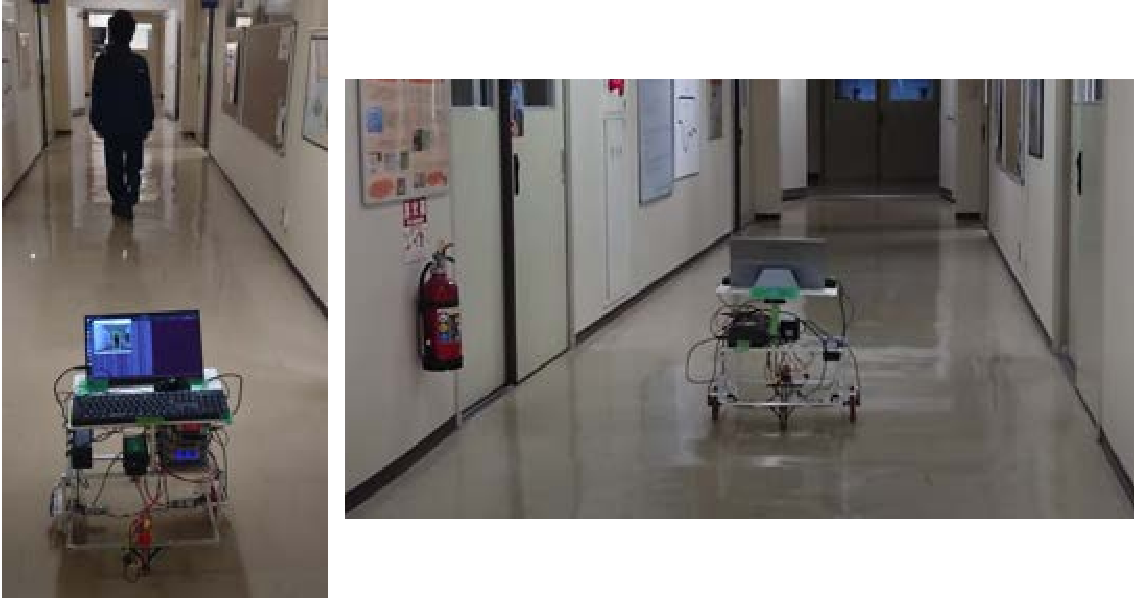
\includegraphics[width=0.8\textwidth]{figure/robo.pdf}
    \caption{実験の様子}
    \label{fig:robo}
\end{figure}

\subsubsection{実験の手順}
各アルゴリズムについて,以下の手順で実験を行った.
\begin{enumerate}
    \item ロボットの前(1[m])に追従物(人)を配置し,カメラの中心に来ていることを確認して実験を始める.
    \item 開始後,人が条件1,2に則り10[m]移動.
    \item エンコーダーデータやカメラデータを記録.
    \item 記録したcsvファイルを解析.
    \item これを3つのアルゴリズム,2つの条件で実験を行う.
\end{enumerate}

\subsection{実験結果及び考察}
本実験では,各アルゴリズム(PN,MPN,GS-MPN)の性能を比較するために,以下の指標を計測した.
\begin{itemize}
    \item \textbf{MeanOffset (px)}: ターゲット中心からの平均オフセット
    \item \textbf{StdOffset (px)}: オフセットの標準偏差
    \item \textbf{MeanAccel (mm/s²)}: 平均加速度
    \item \textbf{StdAccel (mm/s²)}: 加速度の標準偏差
\end{itemize}

表\ref{tab:experiment_results}に,各アルゴリズムの実験結果を示す.
また,図\ref{fig:offset_results}にMeanOffsetとStdOffset,図\ref{fig:accel_results}にMeanAccelとStdAccelのグラフを示す.

\begin{table}[H]
    \centering
    \caption{各アルゴリズムの実験結果}
    \label{tab:experiment_results}
    \resizebox{\textwidth}{!}{%
        \begin{tabular}{|l|c|c|c|c|}
            \hline
            \textbf{Experiment} & \textbf{MeanOffset (px)} & \textbf{StdOffset (px)} & \textbf{MeanAccel (mm/s²)} & \textbf{StdAccel (mm/s²)} \\ \hline
            PN\_data1           & 41.86                    & 54.03                   & 29.08                      & 29109.58                  \\ \hline
            PN\_data2           & 59.89                    & 64.74                   & 128.51                     & 27609.34                  \\ \hline
            MPN\_data1          & 102.42                   & 57.05                   & 202.61                     & 27873.37                  \\ \hline
            MPN\_data2          & 36.15                    & 51.27                   & 55.08                      & 11523.68                  \\ \hline
            GS-MPN\_data1       & 66.29                    & 69.30                   & 101.00                     & 11177.16                  \\ \hline
            GS-MPN\_data2       & 48.94                    & 69.98                   & 50.11                      & 21241.42                  \\ \hline
        \end{tabular}%
    }
\end{table}


\begin{figure}[H]
    \centering
    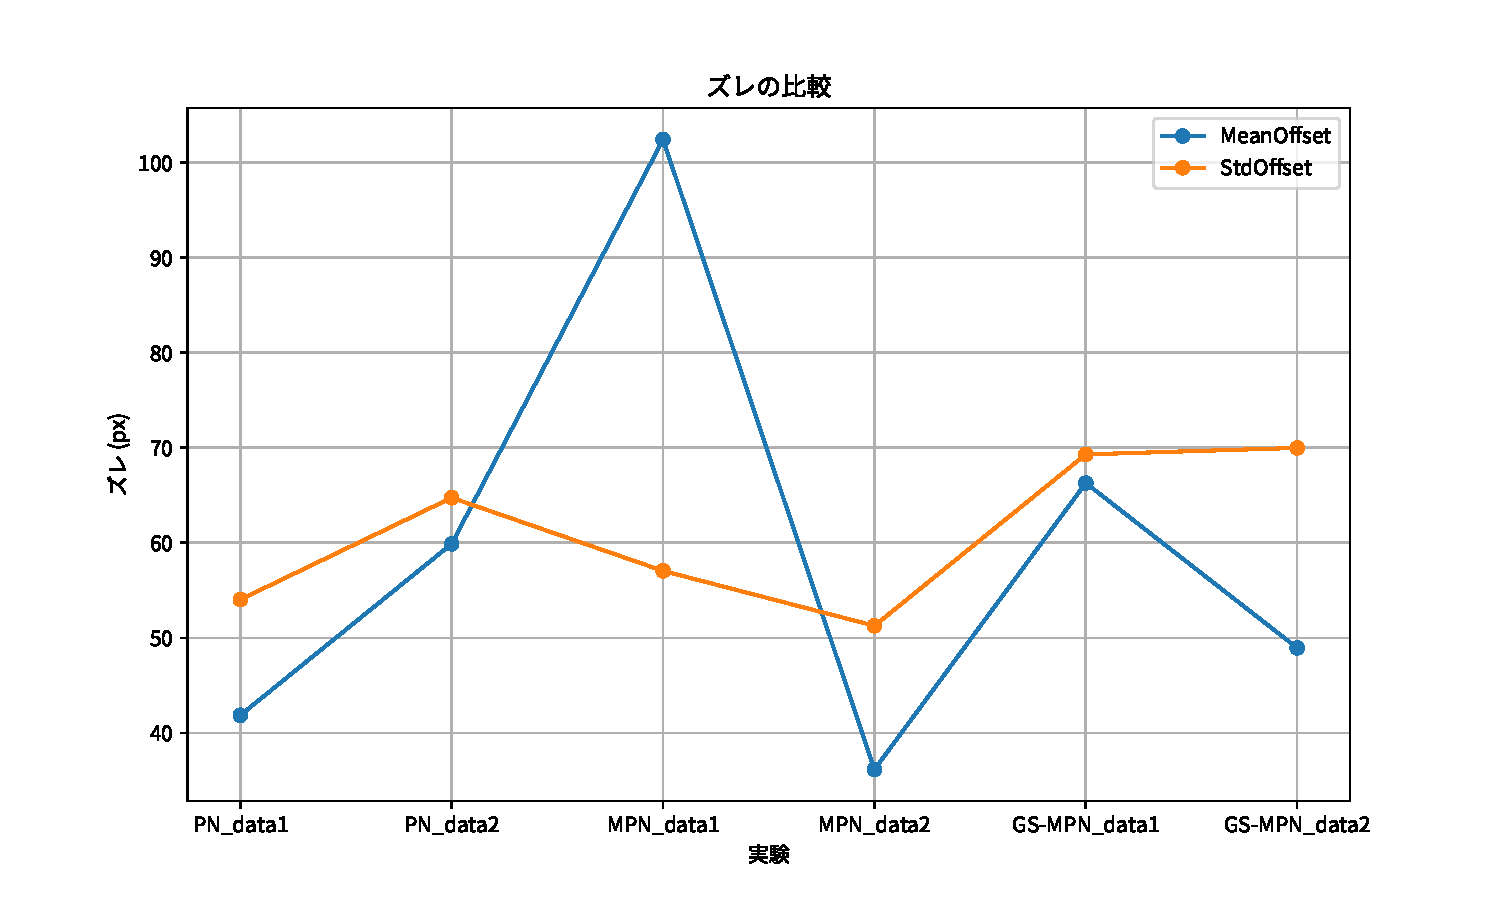
\includegraphics[width=1\textwidth]{figure/Offset.pdf}
    \caption{MeanOffsetおよびStdOffsetの比較}
    \label{fig:offset_results}
\end{figure}

\begin{figure}[H]
    \centering
    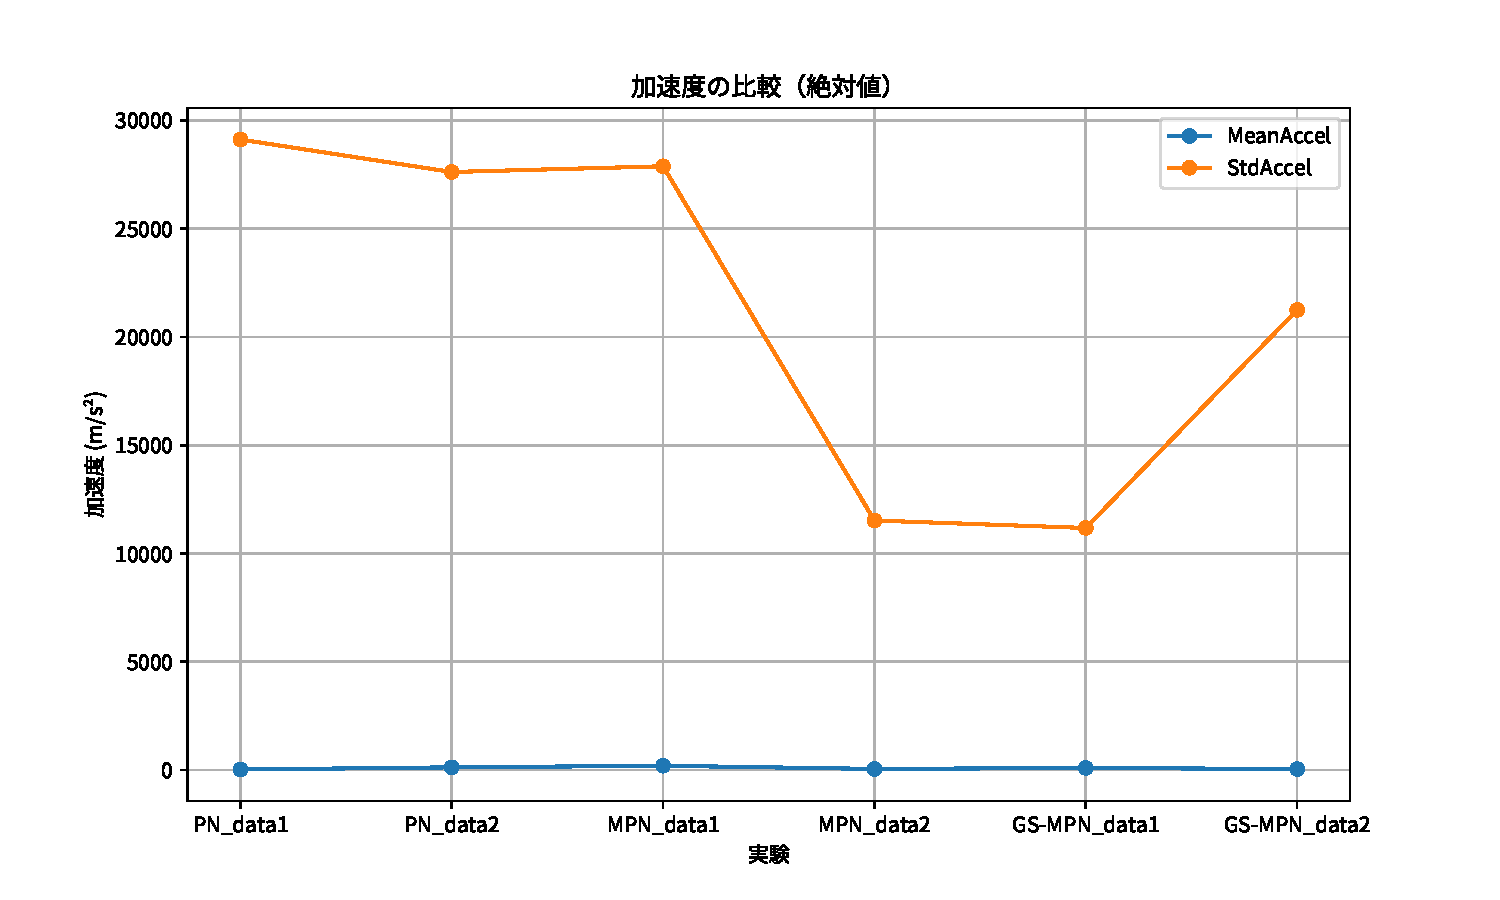
\includegraphics[width=1\textwidth]{figure/Accel.pdf}
    \caption{MeanAccelおよびStdAccelの比較}
    \label{fig:accel_results}
\end{figure}

\subsubsection{追従性能(MeanOffsetとStdOffset)}
追従性能を評価するために,MeanOffset(画面中心からのズレの平均値)とStdOffset(ズレの標準偏差)を用いた.
この指標は,目標物が画面内で中心付近にどれだけ正確に保持されているかを示す.
表\ref{tab:offset_results}に各アルゴリズムの結果を示す.

\begin{table}[H]
    \centering
    \caption{追従性能の評価結果}
    \label{tab:offset_results}
    \begin{tabular}{|l|c|c|}
        \hline
        \textbf{アルゴリズム} & \textbf{MeanOffset (px)} & \textbf{StdOffset (px)} \\ \hline
        PN\_data1             & 41.86                    & 54.03                   \\ \hline
        PN\_data2             & 59.89                    & 64.74                   \\ \hline
        MPN\_data1            & 102.42                   & 57.05                   \\ \hline
        MPN\_data2            & 36.15                    & 51.27                   \\ \hline
        GS-MPN\_data1         & 66.29                    & 69.30                   \\ \hline
        GS-MPN\_data2         & 48.94                    & 69.98                   \\ \hline
    \end{tabular}
\end{table}

PNは直線追従時に最も良好なMeanOffsetを示したが,曲線追従ではズレが大きくなり安定性が低下した.
一方で,MPNとGS-MPNは曲線追従時にズレが減少し,安定性が向上した.
特にGS-MPNは,MeanOffsetとStdOffsetの両方でバランスの良い結果を示している.

\subsubsection{スムーズさ(MeanAccelとStdAccel)}
スムーズさの指標として,MeanAccel(加速度の平均値)とStdAccel(加速度のばらつき)を用いた.
これらはロボットの動作の安定性と滑らかさを評価する.表\ref{tab:accel_results}に結果を示す.

\begin{table}[H]
    \centering
    \caption{スムーズさの評価結果}
    \label{tab:accel_results}
    \begin{tabular}{|l|c|c|}
        \hline
        \textbf{アルゴリズム} & \textbf{MeanAccel (mm/s²)} & \textbf{StdAccel (mm/s²)} \\ \hline
        PN\_data1             & 29.08                      & 29109.58                  \\ \hline
        PN\_data2             & 128.51                     & 27609.34                  \\ \hline
        MPN\_data1            & 202.61                     & 27873.37                  \\ \hline
        MPN\_data2            & 55.08                      & 11523.68                  \\ \hline
        GS-MPN\_data1         & 101.00                     & 11177.16                  \\ \hline
        GS-MPN\_data2         & 50.11                      & 21241.42                  \\ \hline
    \end{tabular}
\end{table}

PNは加速度のばらつき(StdAccel)が非常に大きく,急加速が多発する結果となった.
MPNでは曲線追従時に加速度が抑えられ,StdAccelが減少した.GS-MPNではさらにばらつきが抑えられ,最も滑らかな動作が実現された.

\subsubsection{視野内追従率(InFrameRate)}
視野内追従率(InFrameRate)は,目標物がカメラの視野内に保持されている割合を示す.
すべてのアルゴリズムで視野内追従率は100\%を記録し,目標物が常に視野内に維持されていることが確認された.

\subsubsection{総合評価}
本実験では,各アルゴリズム(PN,MPN,GS-MPN)を対象に追従性能,スムーズさ,および視野内追従率を評価した.

まず,PN(Proportional Navigation)は直線追従性能において最も良好な結果を示した.MeanOffsetが最小値を記録し,
目標物を中心付近に保持する能力が高いことが確認された.
一方で,StdOffsetが増加する傾向があり,特に曲線追従時にはズレが顕著になることが課題として挙げられる.
また,加速度のばらつき(StdAccel)が他のアルゴリズムに比べて極めて大きく,急激な動作が多発する結果となった.
このことから,PNは直線的な動作には適しているものの,動的環境や急な方向転換を必要とする状況では不安定性が課題となる.

次に,MPN(Modified Proportional Navigation)は,PNと比較して曲線追従性能と動作の滑らかさが大幅に改善された.
特にStdAccelの減少により,加速度のばらつきが抑制され,急激な加速や減速が少ない安定した動作が確認された.
さらに,MPN\_data2では,MeanOffsetとStdOffsetの値が他の条件よりも小さく,曲線追従における追従精度と安定性のバランスが良好であることが示されている.
しかしながら,直線追従時にはMeanAccelが最大値を記録しており,急加速が発生する傾向が見られた.
これは,微分項の影響が過大である可能性を示唆しており,直進時の制御パラメータの最適化が求められる.

最後に,GS-MPN(Gain-Scheduled Modified Proportional Navigation)は,全体的に最もバランスの取れた性能を示した.
動的微分ゲインを導入することで,急加速を抑制しながら安定した追従動作を実現していることが,MeanAccelおよびStdAccelの大幅な低下から確認された.
さらに,曲線追従においてもズレが抑制され,MPNよりも安定性が向上している.
一方で,MeanOffsetがPNと比較してやや大きい値を示しており,直線追従精度のさらなる向上が課題として挙げられる.
これには,動的微分ゲインの調整や,追加の制御項を導入することが効果的であると考えられる.

本実験の結果から,GS-MPNは滑らかな追従動作を必要とするシナリオにおいて最も有効であることが示唆された.
直線および曲線追従の両方において安定性が向上し,加速度のばらつきが最小化されることで,ロボットの動作がより自然で滑らかになることが確認された.
一方で,追従精度を向上させるための追加的な制御パラメータの調整や,動的環境における性能検証が今後の研究課題として残されている.
 \newpage
% !TEX root = main.tex
\section{おわりに}
本研究では,カメラのみを用いた人追従搬送ロボットの開発を目指し,Intel RealSense D435iから取得したデータを活用して人の位置を推定し,追従アルゴリズムに基づいてロボットを制御するシステムを構築した.特に,修正比例航法(MPN)やゲインスケジューリング下修正比例航法(GS-MPN)を用いることで,従来の比例航法(PN)では対応が難しかった滑らかな動作や安定性の向上を図った.また,デプスカメラの画像データを用いて物理空間での人の座標を高精度に推定する仕組みを実装し,ロボット制御に反映させた.これにより,低コストなセンサーを使用したロボットシステムの可能性を示すことができた.

本研究の成果として,次の点が挙げられる.まず,PN,MPN,GS-MPNの3つの追従アルゴリズムを比較評価し,GS-MPNが最もバランスの取れた追従性能と動作の滑らかさを実現することを確認した.また,ロボットのハードウェア構成として,D435iを中心としたカメラシステム,STM32を使用した下位制御層,およびROS2による上位制御層を統合したシステムを構築し,それぞれの役割を分担させることで,スムーズなデータ処理と制御を可能にした.さらに,追従性能の評価では,GS-MPNが急加速やズレの少ない安定した追従を実現し,従来手法を上回る性能を示した.

一方で,本研究にはいくつかの課題も残された.まず,カメラの視野内での追従には成功したものの,遮蔽物が発生した場合や複数の対象物が存在する場合における動作安定性については十分に検証が行えていない.特定のターゲットを継続的に追従するための識別アルゴリズムが必要である.さらに,外乱環境下での耐性についても課題が残る.例えば,屋外での風や路面の不整に対する追従性能の検証は未実施であり,システムの実用化に向けてはこれらの外乱要因への対応が求められる.

また,本研究ではカメラのデプスデータのみを用いて追従アルゴリズムを構築したが,さらなる認識精度の向上を目指してセンサーフュージョンを導入することが考えられる.具体的には,LiDARやIMUなど他のセンサー情報を統合することで,環境の多様な条件に対応可能なシステムが構築できると期待される.また,歩行経路の予測を導入することで,人の進行方向に先回りする制御を実現し,応答性を向上させることも今後の課題として挙げられる.
 \newpage

%%%%%%%%%%%%%%%%%%%%%%%%%%%%%%%%%%%%%%%%%%%%%%%%%%%%%%%%%%%%%%%%%%%%%%%%%%%%%
%%%%%% 参考文献 %%%%%%%%%%%%%%%%%%%%%%%%%%%%%%%%%%%%%%%%%%%%%%%%%%%%%%%%%%%
%%%%%%%%%%%%%%%%%%%%%%%%%%%%%%%%%%%%%%%%%%%%%%%%%%%%%%%%%%%%%%%%%%%%%%%%%%%%%
% !TEX root = main.tex
%%%%%%%%%%%%%%%%%%%%%%%%%%%%%%%%%%%%%%%%%%%%%%%%%%%%%%%%%%%%%%%%%%%%%%%%
\begin{center}
	\section*{\kintou{5zw}{参考文献}}                      %% ここに番号をつけない
	\vspace*{-2zh}
\end{center}
\addcontentsline{toc}{section}{参考文献} %% 目次に番号をつけない
%%%%%%%%%%%%%%%%%%%%%%%%%%%%%%%%%%%%%%%%%%%%%%%%%%%%%%%%%%%%%%%%%%%%%%%%

\begin{thebibliography}{99}
	
	\bibitem{roshon}
	出村 公成, 萩原 良信, 升谷 保博, タン ジェフリー トゥ チュアン
	:ROS2とPythonで作って学ぶAIロボット入門, 
	講談社 (2018)
	
	\bibitem{ros2design}
	ROS 2 Design Documents: \url{https://design.ros2.org/}, [Accessed: Dec. 25, 2024].
	
	\bibitem{ros2docs}
	ROS 2 Documentation: \url{https://docs.ros.org/en/humble/index.html}, [Accessed: Dec. 25, 2024].
	
	\bibitem{yolo}
	ultralytics: \url{https://docs.ultralytics.com/ja/yolov5/}, [Accessed: Dec. 25, 2024].
	
	\bibitem{Saref1to1}
	佐藤太郎:
	高等専門学校における一般科目と専門科目,
	京都出版 (2018)
	\textcolor{red}{\quad\cdotfill\ 本の場合}
	
	\bibitem{Suzuki1}
	鈴木次郎,高橋三郎:
	高等専門学校と大学の違い,
	電子制御学会論文誌,
	Vol.~25, No.~13, 123/130 (2017)
	\textcolor{red}{\quad\cdotfill\ 学会誌論文の場合}
	
	\bibitem{Tanaka1}
	田中史朗,伊藤五郎,渡辺花子:
	高専における就職活動,
	電気電子工学講演会資料,
	543/546 (2016)
	\textcolor{red}{\quad\cdotfill\ 講演会等資料(ページが記載されているもの)の場合}
	
	\bibitem{Yamamoto1}
	山本一二三,中村五十六:
	高専における就職活動,
	メカトロニクス講演会資料,
	全 4 頁 (2016)
	\textcolor{red}{\quad\cdotfill\ 講演会等資料(ページが記載されていないもの)の場合}
	
	\bibitem{Nakamura1}
	中村十三子:
	機械加工と実習工場,
	平成 29 年度舞鶴工業高等専門学校機械工学科卒業論文 (2018)
	\textcolor{red}{\quad\cdotfill\ 卒業論文の場合}
	
	\bibitem{Sato2}
	T.~Sato: 
	General Subjects and Special subjects at National Institute of Technology, 
	Kyoto Publishing (2018)
	
	\bibitem{Suzuki2}
	J.~Suzuki and S.~Takahashi: 
	Difference between National Institute of Technology and Universities, 
	Journal of the Electronic Control Society, 
	Vol.~25, No.~13, 123/130 (2017)
	
	\bibitem{Tanaka2}
	S.~Tanaka, G.~Ito and H.~Watanabe: 
	Job Hunting in NIT, 
	Proceedings of Conference on Electrical and Electronics Engineering, 
	543/546 (2016)
	
	\bibitem{Yamamoto2}
	H.~Yamamoto and I.~Nakamura: 
	Job Hunting in NIT, 
	Proceedings of Mechatoronics Conference, 
	4 pages (2016)
	
	\bibitem{NIT1}
	舞鶴高専ホームページ:
	\url{http://www.maizuru-ct.ac.jp}
\end{thebibliography}
% ******************************************* \newpage

%%%%%%%%%%%%%%%%%%%%%%%%%%%%%%%%%%%%%%%%%%%%%%%%%%%%%%%%%%%%%%%%%%%%%%%%%%%%%
%%%%%% 謝辞 %%%%%%%%%%%%%%%%%%%%%%%%%%%%%%%%%%%%%%%%%%%%%%%%%%%%%%%%%%%%%%%
%%%%%%%%%%%%%%%%%%%%%%%%%%%%%%%%%%%%%%%%%%%%%%%%%%%%%%%%%%%%%%%%%%%%%%%%%%%%%
% !TEX root = main.tex
%%%%%%%%%%%%%%%%%%%%%%%%%%%%%%%%%%%%%%%%%%%%%%%%%%%%%%%%%%%%%%%%%%%%%%%%
\begin{center}
    \section*{\kintou{2.5zw}{謝辞}}                      %% ここに番号をつけない
    \vspace*{-2zh}
\end{center}
\addcontentsline{toc}{section}{謝辞} %% 目次に番号をつけない
%%%%%%%%%%%%%%%%%%%%%%%%%%%%%%%%%%%%%%%%%%%%%%%%%%%%%%%%%%%%%%%%%%%%%%%%

この研究を遂行するにあたり,終始暖かく見守って下さった高木太郎教授に深く感謝いたします。
 \newpage

%%%%%%%%%%%%%%%%%%%%%%%%%%%%%%%%%%%%%%%%%%%%%%%%%%%%%%%%%%%%%%%%%%%%%%%%%%%%%
%%%%%% 付録 %%%%%%%%%%%%%%%%%%%%%%%%%%%%%%%%%%%%%%%%%%%%%%%%%%%%%%%%%%%%%%%
%%%%%%%%%%%%%%%%%%%%%%%%%%%%%%%%%%%%%%%%%%%%%%%%%%%%%%%%%%%%%%%%%%%%%%%%%%%%%
% !TEX root = main.tex
%////////////////////////////////////////////////////////
\begin{center}
    \section*{\kintou{2.5zw}{付録}}                      %% ここに番号をつけない
    \vspace*{-2zh}
\end{center}
\addcontentsline{toc}{section}{付録} %% 目次に番号をつけない
\appendix

\setcounter{equation}{0}
\setcounter{figure}{0}
\setcounter{table}{0}

\makeatletter
     \renewcommand{\theequation}{%
          A.\arabic{equation}}
     \@addtoreset{equation}{section}
\makeatother

\makeatletter
     \renewcommand{\thetable}{%
          A.\arabic{table}}
     \@addtoreset{table}{section}
\makeatother

\makeatletter
     \renewcommand{\thefigure}{%
          A.\arabic{figure}}
     \@addtoreset{figure}{section}
\makeatother

% ================================================
\makeatletter
     \renewcommand{\thesubsection}{%
          A.\arabic{subsection}}
     \@addtoreset{subsection}{section}
\makeatother

\makeatletter
     \renewcommand{\thesubsubsection}{%
          A.\arabic{subsection}.\arabic{subsubsection}}
     \@addtoreset{subsubsection}{section}
\makeatother

% ================================================
\makeatletter
     \renewcommand{\thetheorem}{%
          A.\arabic{theorem}}
     \@addtoreset{theorem}{section}
\makeatother

\makeatletter
     \renewcommand{\thedefinition}{%
          A.\arabic{definition}}
     \@addtoreset{definition}{section}
\makeatother

\makeatletter
     \renewcommand{\thelemma}{%
          A.\arabic{lemma}}
     \@addtoreset{lemma}{section}
\makeatother

\makeatletter
     \renewcommand{\thelstlisting}{%
          {\bf{A.\arabic{lstlisting}}}}
     \@addtoreset{lstlisting}{section}
\makeatother






%////////////////////////////////////////////////////////

%%%%%%%%%%%%%%%%%%%%%%%%%%%%%%%%%%%%%%%%%%%%%%%%%%%%%%
\subsection{下位レイヤープログラム}
%%%%%%%%%%%%%%%%%%%%%%%%%%%%%%%%%%%%%%%%%%%%%%%%%%%%%%

作成したプログラムを以下に示す.
また,\url{https://github.com/Altairu/2_wheel_PID_control-_CubeIED}に掲載している.

\subsubsection{メインプログラム}

\begin{lstlisting}[language=C, caption=メインコード(main.c)]
    #include "main.h"
    #include "motor_driver.h"
    #include "encoder.h"
    #include "serial_lib.h"
    
    TIM_HandleTypeDef htim1;
    TIM_HandleTypeDef htim12;
    TIM_HandleTypeDef htim4;
    TIM_HandleTypeDef htim8;
    UART_HandleTypeDef huart2;
    
    MotorDriver motorRight, motorLeft;
    Encoder encoderRight, encoderLeft;
    EncoderData encoderDataRight, encoderDataLeft;
    
    #define WHEEL_DIAMETER_MM 365 //129.5
    #define ENCODER_PULSES_PER_REV 4096
    
    int16_t controlSignalRight = 0;
    int16_t controlSignalLeft = 0;
    
    void SystemClock_Config(void);
    static void MX_GPIO_Init(void);
    static void MX_USART2_UART_Init(void);
    static void MX_TIM1_Init(void);
    static void MX_TIM12_Init(void);
    static void MX_TIM4_Init(void);
    static void MX_TIM8_Init(void);
    
    int main(void)
    {
        HAL_Init();
        SystemClock_Config();
        MX_GPIO_Init();
        MX_USART2_UART_Init();
        MX_TIM1_Init();
        MX_TIM12_Init();
        MX_TIM4_Init();
        MX_TIM8_Init();
    
        Serial_Init(&huart2);
        MotorDriver_Init(&motorRight, &htim12, TIM_CHANNEL_1, &htim12, TIM_CHANNEL_2);
        MotorDriver_Init(&motorLeft, &htim1, TIM_CHANNEL_4, &htim1, TIM_CHANNEL_1);
        Encoder_Init(&encoderRight, &htim8, WHEEL_DIAMETER_MM, ENCODER_PULSES_PER_REV, 10);
        Encoder_Init(&encoderLeft, &htim4, WHEEL_DIAMETER_MM, ENCODER_PULSES_PER_REV, 10);
    
        uint32_t lastSendTime = HAL_GetTick();
    
        while (1)
        {
            /* PCからの制御信号を受信 */
            int16_t receivedData[2];
            if (Serial_ReceiveData(&huart2, receivedData, 2))
            {
                controlSignalRight = receivedData[0];
                controlSignalLeft = receivedData[1];
    
                MotorDriver_setSpeed(&motorRight, -1* controlSignalRight);
                MotorDriver_setSpeed(&motorLeft,   controlSignalLeft);
            }
    
            /* エンコーダーデータの送信(10msごとに送信) */
            if (HAL_GetTick() - lastSendTime >= 10)
            {
                lastSendTime = HAL_GetTick();
    
                /* エンコーダーの速度データを更新 */
                Encoder_Interrupt(&encoderRight, &encoderDataRight);
                Encoder_Interrupt(&encoderLeft, &encoderDataLeft);
    
                /* エンコーダー速度を送信 */
                int16_t feedbackData[2] = {(int16_t)encoderDataRight.velocity, -1*(int16_t)encoderDataLeft.velocity};
                Serial_SendData(&huart2, feedbackData, 2);
            }
        }
    }
    
    
    /**
      * @brief System Clock Configuration
      * @retval None
      */
    void SystemClock_Config(void)
    {
      RCC_OscInitTypeDef RCC_OscInitStruct = {0};
      RCC_ClkInitTypeDef RCC_ClkInitStruct = {0};
    
      /** Configure the main internal regulator output voltage
      */
      __HAL_RCC_PWR_CLK_ENABLE();
      __HAL_PWR_VOLTAGESCALING_CONFIG(PWR_REGULATOR_VOLTAGE_SCALE3);
    
      /** Initializes the RCC Oscillators according to the specified parameters
      * in the RCC_OscInitTypeDef structure.
      */
      RCC_OscInitStruct.OscillatorType = RCC_OSCILLATORTYPE_HSI;
      RCC_OscInitStruct.HSIState = RCC_HSI_ON;
      RCC_OscInitStruct.HSICalibrationValue = RCC_HSICALIBRATION_DEFAULT;
      RCC_OscInitStruct.PLL.PLLState = RCC_PLL_ON;
      RCC_OscInitStruct.PLL.PLLSource = RCC_PLLSOURCE_HSI;
      RCC_OscInitStruct.PLL.PLLM = 16;
      RCC_OscInitStruct.PLL.PLLN = 336;
      RCC_OscInitStruct.PLL.PLLP = RCC_PLLP_DIV4;
      RCC_OscInitStruct.PLL.PLLQ = 2;
      RCC_OscInitStruct.PLL.PLLR = 2;
      if (HAL_RCC_OscConfig(&RCC_OscInitStruct) != HAL_OK)
      {
        Error_Handler();
      }
    
      /** Initializes the CPU, AHB and APB buses clocks
      */
      RCC_ClkInitStruct.ClockType = RCC_CLOCKTYPE_HCLK|RCC_CLOCKTYPE_SYSCLK
                                  |RCC_CLOCKTYPE_PCLK1|RCC_CLOCKTYPE_PCLK2;
      RCC_ClkInitStruct.SYSCLKSource = RCC_SYSCLKSOURCE_PLLCLK;
      RCC_ClkInitStruct.AHBCLKDivider = RCC_SYSCLK_DIV1;
      RCC_ClkInitStruct.APB1CLKDivider = RCC_HCLK_DIV2;
      RCC_ClkInitStruct.APB2CLKDivider = RCC_HCLK_DIV1;
    
      if (HAL_RCC_ClockConfig(&RCC_ClkInitStruct, FLASH_LATENCY_2) != HAL_OK)
      {
        Error_Handler();
      }
    }
    
    /**
      * @brief TIM1 Initialization Function
      * @param None
      * @retval None
      */
    static void MX_TIM1_Init(void)
    {
    
      /* USER CODE BEGIN TIM1_Init 0 */
    
      /* USER CODE END TIM1_Init 0 */
    
      TIM_MasterConfigTypeDef sMasterConfig = {0};
      TIM_OC_InitTypeDef sConfigOC = {0};
      TIM_BreakDeadTimeConfigTypeDef sBreakDeadTimeConfig = {0};
    
      /* USER CODE BEGIN TIM1_Init 1 */
    
      /* USER CODE END TIM1_Init 1 */
      htim1.Instance = TIM1;
      htim1.Init.Prescaler = 0;
      htim1.Init.CounterMode = TIM_COUNTERMODE_UP;
      htim1.Init.Period = 65535;
      htim1.Init.ClockDivision = TIM_CLOCKDIVISION_DIV1;
      htim1.Init.RepetitionCounter = 0;
      htim1.Init.AutoReloadPreload = TIM_AUTORELOAD_PRELOAD_DISABLE;
      if (HAL_TIM_PWM_Init(&htim1) != HAL_OK)
      {
        Error_Handler();
      }
      sMasterConfig.MasterOutputTrigger = TIM_TRGO_RESET;
      sMasterConfig.MasterSlaveMode = TIM_MASTERSLAVEMODE_DISABLE;
      if (HAL_TIMEx_MasterConfigSynchronization(&htim1, &sMasterConfig) != HAL_OK)
      {
        Error_Handler();
      }
      sConfigOC.OCMode = TIM_OCMODE_PWM1;
      sConfigOC.Pulse = 0;
      sConfigOC.OCPolarity = TIM_OCPOLARITY_HIGH;
      sConfigOC.OCNPolarity = TIM_OCNPOLARITY_HIGH;
      sConfigOC.OCFastMode = TIM_OCFAST_DISABLE;
      sConfigOC.OCIdleState = TIM_OCIDLESTATE_RESET;
      sConfigOC.OCNIdleState = TIM_OCNIDLESTATE_RESET;
      if (HAL_TIM_PWM_ConfigChannel(&htim1, &sConfigOC, TIM_CHANNEL_1) != HAL_OK)
      {
        Error_Handler();
      }
      if (HAL_TIM_PWM_ConfigChannel(&htim1, &sConfigOC, TIM_CHANNEL_4) != HAL_OK)
      {
        Error_Handler();
      }
      sBreakDeadTimeConfig.OffStateRunMode = TIM_OSSR_DISABLE;
      sBreakDeadTimeConfig.OffStateIDLEMode = TIM_OSSI_DISABLE;
      sBreakDeadTimeConfig.LockLevel = TIM_LOCKLEVEL_OFF;
      sBreakDeadTimeConfig.DeadTime = 0;
      sBreakDeadTimeConfig.BreakState = TIM_BREAK_DISABLE;
      sBreakDeadTimeConfig.BreakPolarity = TIM_BREAKPOLARITY_HIGH;
      sBreakDeadTimeConfig.AutomaticOutput = TIM_AUTOMATICOUTPUT_DISABLE;
      if (HAL_TIMEx_ConfigBreakDeadTime(&htim1, &sBreakDeadTimeConfig) != HAL_OK)
      {
        Error_Handler();
      }
      /* USER CODE BEGIN TIM1_Init 2 */
    
      /* USER CODE END TIM1_Init 2 */
      HAL_TIM_MspPostInit(&htim1);
    
    }
    
    /**
      * @brief TIM4 Initialization Function
      * @param None
      * @retval None
      */
    static void MX_TIM4_Init(void)
    {
    
      /* USER CODE BEGIN TIM4_Init 0 */
    
      /* USER CODE END TIM4_Init 0 */
    
      TIM_Encoder_InitTypeDef sConfig = {0};
      TIM_MasterConfigTypeDef sMasterConfig = {0};
    
      /* USER CODE BEGIN TIM4_Init 1 */
    
      /* USER CODE END TIM4_Init 1 */
      htim4.Instance = TIM4;
      htim4.Init.Prescaler = 0;
      htim4.Init.CounterMode = TIM_COUNTERMODE_UP;
      htim4.Init.Period = 65535;
      htim4.Init.ClockDivision = TIM_CLOCKDIVISION_DIV1;
      htim4.Init.AutoReloadPreload = TIM_AUTORELOAD_PRELOAD_DISABLE;
      sConfig.EncoderMode = TIM_ENCODERMODE_TI1;
      sConfig.IC1Polarity = TIM_ICPOLARITY_RISING;
      sConfig.IC1Selection = TIM_ICSELECTION_DIRECTTI;
      sConfig.IC1Prescaler = TIM_ICPSC_DIV1;
      sConfig.IC1Filter = 0;
      sConfig.IC2Polarity = TIM_ICPOLARITY_RISING;
      sConfig.IC2Selection = TIM_ICSELECTION_DIRECTTI;
      sConfig.IC2Prescaler = TIM_ICPSC_DIV1;
      sConfig.IC2Filter = 0;
      if (HAL_TIM_Encoder_Init(&htim4, &sConfig) != HAL_OK)
      {
        Error_Handler();
      }
      sMasterConfig.MasterOutputTrigger = TIM_TRGO_RESET;
      sMasterConfig.MasterSlaveMode = TIM_MASTERSLAVEMODE_DISABLE;
      if (HAL_TIMEx_MasterConfigSynchronization(&htim4, &sMasterConfig) != HAL_OK)
      {
        Error_Handler();
      }
      /* USER CODE BEGIN TIM4_Init 2 */
    
      /* USER CODE END TIM4_Init 2 */
    
    }
    
    /**
      * @brief TIM8 Initialization Function
      * @param None
      * @retval None
      */
    static void MX_TIM8_Init(void)
    {
    
      /* USER CODE BEGIN TIM8_Init 0 */
    
      /* USER CODE END TIM8_Init 0 */
    
      TIM_Encoder_InitTypeDef sConfig = {0};
      TIM_MasterConfigTypeDef sMasterConfig = {0};
    
      /* USER CODE BEGIN TIM8_Init 1 */
    
      /* USER CODE END TIM8_Init 1 */
      htim8.Instance = TIM8;
      htim8.Init.Prescaler = 0;
      htim8.Init.CounterMode = TIM_COUNTERMODE_UP;
      htim8.Init.Period = 65535;
      htim8.Init.ClockDivision = TIM_CLOCKDIVISION_DIV1;
      htim8.Init.RepetitionCounter = 0;
      htim8.Init.AutoReloadPreload = TIM_AUTORELOAD_PRELOAD_DISABLE;
      sConfig.EncoderMode = TIM_ENCODERMODE_TI1;
      sConfig.IC1Polarity = TIM_ICPOLARITY_RISING;
      sConfig.IC1Selection = TIM_ICSELECTION_DIRECTTI;
      sConfig.IC1Prescaler = TIM_ICPSC_DIV1;
      sConfig.IC1Filter = 0;
      sConfig.IC2Polarity = TIM_ICPOLARITY_RISING;
      sConfig.IC2Selection = TIM_ICSELECTION_DIRECTTI;
      sConfig.IC2Prescaler = TIM_ICPSC_DIV1;
      sConfig.IC2Filter = 0;
      if (HAL_TIM_Encoder_Init(&htim8, &sConfig) != HAL_OK)
      {
        Error_Handler();
      }
      sMasterConfig.MasterOutputTrigger = TIM_TRGO_RESET;
      sMasterConfig.MasterSlaveMode = TIM_MASTERSLAVEMODE_DISABLE;
      if (HAL_TIMEx_MasterConfigSynchronization(&htim8, &sMasterConfig) != HAL_OK)
      {
        Error_Handler();
      }
      /* USER CODE BEGIN TIM8_Init 2 */
    
      /* USER CODE END TIM8_Init 2 */
    
    }
    
    /**
      * @brief TIM12 Initialization Function
      * @param None
      * @retval None
      */
    static void MX_TIM12_Init(void)
    {
    
      /* USER CODE BEGIN TIM12_Init 0 */
    
      /* USER CODE END TIM12_Init 0 */
    
      TIM_OC_InitTypeDef sConfigOC = {0};
    
      /* USER CODE BEGIN TIM12_Init 1 */
    
      /* USER CODE END TIM12_Init 1 */
      htim12.Instance = TIM12;
      htim12.Init.Prescaler = 0;
      htim12.Init.CounterMode = TIM_COUNTERMODE_UP;
      htim12.Init.Period = 65535;
      htim12.Init.ClockDivision = TIM_CLOCKDIVISION_DIV1;
      htim12.Init.AutoReloadPreload = TIM_AUTORELOAD_PRELOAD_DISABLE;
      if (HAL_TIM_PWM_Init(&htim12) != HAL_OK)
      {
        Error_Handler();
      }
      sConfigOC.OCMode = TIM_OCMODE_PWM1;
      sConfigOC.Pulse = 0;
      sConfigOC.OCPolarity = TIM_OCPOLARITY_HIGH;
      sConfigOC.OCFastMode = TIM_OCFAST_DISABLE;
      if (HAL_TIM_PWM_ConfigChannel(&htim12, &sConfigOC, TIM_CHANNEL_1) != HAL_OK)
      {
        Error_Handler();
      }
      if (HAL_TIM_PWM_ConfigChannel(&htim12, &sConfigOC, TIM_CHANNEL_2) != HAL_OK)
      {
        Error_Handler();
      }
      /* USER CODE BEGIN TIM12_Init 2 */
    
      /* USER CODE END TIM12_Init 2 */
      HAL_TIM_MspPostInit(&htim12);
    
    }
    
    /**
      * @brief USART2 Initialization Function
      * @param None
      * @retval None
      */
    static void MX_USART2_UART_Init(void)
    {
    
      /* USER CODE BEGIN USART2_Init 0 */
    
      /* USER CODE END USART2_Init 0 */
    
      /* USER CODE BEGIN USART2_Init 1 */
    
      /* USER CODE END USART2_Init 1 */
      huart2.Instance = USART2;
      huart2.Init.BaudRate = 115200;
      huart2.Init.WordLength = UART_WORDLENGTH_8B;
      huart2.Init.StopBits = UART_STOPBITS_1;
      huart2.Init.Parity = UART_PARITY_NONE;
      huart2.Init.Mode = UART_MODE_TX_RX;
      huart2.Init.HwFlowCtl = UART_HWCONTROL_NONE;
      huart2.Init.OverSampling = UART_OVERSAMPLING_16;
      if (HAL_UART_Init(&huart2) != HAL_OK)
      {
        Error_Handler();
      }
      /* USER CODE BEGIN USART2_Init 2 */
    
      /* USER CODE END USART2_Init 2 */
    
    }
    
    /**
      * @brief GPIO Initialization Function
      * @param None
      * @retval None
      */
    static void MX_GPIO_Init(void)
    {
      GPIO_InitTypeDef GPIO_InitStruct = {0};
    /* USER CODE BEGIN MX_GPIO_Init_1 */
    /* USER CODE END MX_GPIO_Init_1 */
    
      /* GPIO Ports Clock Enable */
      __HAL_RCC_GPIOC_CLK_ENABLE();
      __HAL_RCC_GPIOH_CLK_ENABLE();
      __HAL_RCC_GPIOA_CLK_ENABLE();
      __HAL_RCC_GPIOB_CLK_ENABLE();
    
      /*Configure GPIO pin Output Level */
      HAL_GPIO_WritePin(LED_GPIO_Port, LED_Pin, GPIO_PIN_RESET);
    
      /*Configure GPIO pin : B1_Pin */
      GPIO_InitStruct.Pin = B1_Pin;
      GPIO_InitStruct.Mode = GPIO_MODE_IT_FALLING;
      GPIO_InitStruct.Pull = GPIO_NOPULL;
      HAL_GPIO_Init(B1_GPIO_Port, &GPIO_InitStruct);
    
      /*Configure GPIO pin : LED_Pin */
      GPIO_InitStruct.Pin = LED_Pin;
      GPIO_InitStruct.Mode = GPIO_MODE_OUTPUT_PP;
      GPIO_InitStruct.Pull = GPIO_NOPULL;
      GPIO_InitStruct.Speed = GPIO_SPEED_FREQ_LOW;
      HAL_GPIO_Init(LED_GPIO_Port, &GPIO_InitStruct);
    
    /* USER CODE BEGIN MX_GPIO_Init_2 */
    /* USER CODE END MX_GPIO_Init_2 */
    }
    
    /* USER CODE BEGIN 4 */
    
    /* USER CODE END 4 */
    
    /**
      * @brief  This function is executed in case of error occurrence.
      * @retval None
      */
    void Error_Handler(void)
    {
      /* USER CODE BEGIN Error_Handler_Debug */
      /* User can add his own implementation to report the HAL error return state */
      __disable_irq();
      while (1)
      {
      }
      /* USER CODE END Error_Handler_Debug */
    }
    
    #ifdef  USE_FULL_ASSERT
    /**
      * @brief  Reports the name of the source file and the source line number
      *         where the assert_param error has occurred.
      * @param  file: pointer to the source file name
      * @param  line: assert_param error line source number
      * @retval None
      */
    void assert_failed(uint8_t *file, uint32_t line)
    {
      /* USER CODE BEGIN 6 */
      /* User can add his own implementation to report the file name and line number,
         ex: printf("Wrong parameters value: file %s on line %d\r\n", file, line) */
      /* USER CODE END 6 */
    }
    #endif /* USE_FULL_ASSERT */

\end{lstlisting}

\subsubsection{エンコーダーライブラリ}

\begin{lstlisting}[language=C, caption=エンコーダーライブラリ(encoder.h)]
    // kinematics.h

    #ifndef KINEMATICS_H
    #define KINEMATICS_H
    
    typedef enum {
        OMNI_3,
        OMNI_4,
        MEKANUM
    } WheelMode;
    
    typedef struct {
        float robot_diameter;   // ロボットの直径
        float wheel_radius;     // ホイールの半径
        WheelMode mode;         // 動作モード
    } Kinematics;
    
    // 初期化関数
    void Kinematics_Init(Kinematics *kinematics, float robot_diameter, float wheel_radius, WheelMode mode);
    
    // モーターの目標速度を計算する関数
    void Kinematics_GetTargetSpeeds(Kinematics *kinematics, float lx, float ly, float rx, float *speedFR, float *speedFL, float *speedBR, float *speedBL);
    
    #endif // KINEMATICS_H
\end{lstlisting}

\begin{lstlisting}[language=C, caption=エンコーダーライブラリ(encoder.c)]
    #include "encoder.h"

    #define TIMER_MAX_COUNT 65535  // タイマーの最大値( 16 ビットタイマーの場合)
    
    void Encoder_Init(Encoder* encoder, TIM_HandleTypeDef* htim, double diameter, int ppr, int period)
    {
        encoder->htim = htim;
        encoder->ppr = ppr;
        encoder->diameter = diameter;
        encoder->period = period;
        encoder->limit = 0;
        encoder->before_rot = 0.0;
    
        encoder->htim->Init.Prescaler = 0;
        encoder->htim->Init.CounterMode = TIM_COUNTERMODE_UP;
        encoder->htim->Init.Period = TIMER_MAX_COUNT;
        encoder->htim->Init.ClockDivision = TIM_CLOCKDIVISION_DIV1;
    
        TIM_Encoder_InitTypeDef encoder_init;
        encoder_init.EncoderMode = TIM_ENCODERMODE_TI12;
        encoder_init.IC1Polarity = TIM_ICPOLARITY_RISING;
        encoder_init.IC1Selection = TIM_ICSELECTION_DIRECTTI;
        encoder_init.IC1Prescaler = TIM_ICPSC_DIV1;
        encoder_init.IC1Filter = 0;
        encoder_init.IC2Polarity = TIM_ICPOLARITY_RISING;
        encoder_init.IC2Selection = TIM_ICSELECTION_DIRECTTI;
        encoder_init.IC2Prescaler = TIM_ICPSC_DIV1;
        encoder_init.IC2Filter = 0;
    
        HAL_TIM_Encoder_Init(htim, &encoder_init);
        HAL_TIM_Encoder_Start(htim, TIM_CHANNEL_ALL);
        __HAL_TIM_SET_COUNTER(htim, TIMER_MAX_COUNT / 2);  // カウンタを中央に設定
    }
    
    int Encoder_Read(Encoder* encoder)
    {
        int16_t count = (int16_t)(__HAL_TIM_GET_COUNTER(encoder->htim) - TIMER_MAX_COUNT / 2);
        return count;
    }
    
    void Encoder_Interrupt(Encoder* encoder, EncoderData* encoder_data)
    {
        int count = Encoder_Read(encoder);
    
        encoder_data->count = count;
        encoder_data->rot = count / (double)encoder->ppr;
        encoder_data->deg = encoder_data->rot * 360.0;
        encoder_data->distance = encoder_data->rot * (PI * encoder->diameter);
    
        encoder_data->rps = (encoder_data->rot - encoder->before_rot) / (encoder->period * 0.001);
        encoder_data->velocity = encoder_data->rps * PI * encoder->diameter;
    
        encoder->before_rot = encoder_data->rot;
    }
    
    void Encoder_Reset(Encoder* encoder)
    {
        __HAL_TIM_SET_COUNTER(encoder->htim, TIMER_MAX_COUNT / 2);  // カウンタを中央にリセット
    }
\end{lstlisting}

\subsubsection{モータドライバーライブラリ}

\begin{lstlisting}[language=C, caption=モータドライバーライブラリ(motor\_driver.h)]
    #ifndef MOTOR_DRIVER_H
    #define MOTOR_DRIVER_H
    
    #include "stm32f4xx_hal.h"
    
    typedef struct {
        TIM_HandleTypeDef* htimA;  // タイマーA
        uint32_t channelA;         // タイマーチャンネルA
        TIM_HandleTypeDef* htimB;  // タイマーB
        uint32_t channelB;         // タイマーチャンネルB
    } MotorDriver;
    
    // モータードライバを初期化する関数
    void MotorDriver_Init(MotorDriver* motor, TIM_HandleTypeDef* htimA, uint32_t channelA,
                          TIM_HandleTypeDef* htimB, uint32_t channelB);
    
    // モーターの速度を設定する関数
    void MotorDriver_setSpeed(MotorDriver* motor, int speed);
    
    #endif /* MOTOR_DRIVER_H */
\end{lstlisting}

\begin{lstlisting}[language=C, caption=モータドライバーライブラリ(motor\_driver.c)]
    #include "motor_driver.h"

    // 初期化関数
    void MotorDriver_Init(MotorDriver* motor, TIM_HandleTypeDef* htimA, uint32_t channelA,
                          TIM_HandleTypeDef* htimB, uint32_t channelB) {
        motor->htimA = htimA;
        motor->channelA = channelA;
        motor->htimB = htimB;
        motor->channelB = channelB;
    
        // PWM 開始
        HAL_TIM_PWM_Start(htimA, channelA);
        HAL_TIM_PWM_Start(htimB, channelB);
    }
    
    // 速度設定関数
    void MotorDriver_setSpeed(MotorDriver *motor, int speed) {
        int pwm_value;
        if (speed > 100) speed = 99;
        if (speed < -100) speed = -99;
    
        if (speed > 0) {
            pwm_value = (speed * __HAL_TIM_GET_AUTORELOAD(motor->htimA)) / 100;
            __HAL_TIM_SET_COMPARE(motor->htimA, motor->channelA, pwm_value);
            __HAL_TIM_SET_COMPARE(motor->htimB, motor->channelB, 0);
        } else {
            pwm_value = (-speed * __HAL_TIM_GET_AUTORELOAD(motor->htimA)) / 100;
            __HAL_TIM_SET_COMPARE(motor->htimA, motor->channelA, 0);
            __HAL_TIM_SET_COMPARE(motor->htimB, motor->channelB, pwm_value);
        }
    }
\end{lstlisting}

\subsubsection{シリアル通信ライブラリ}

\begin{lstlisting}[language=C, caption=シリアル通信ライブラリ(serial\_lib.h)]
    #ifndef SERIAL_LIB_H
    #define SERIAL_LIB_H
    
    #include "main.h"
    
    // シリアルヘッダーの定義
    #define SERIAL_HEADER1 0xA5
    #define SERIAL_HEADER2 0xA5
    
    // 関数プロトタイプ
    void Serial_Init(UART_HandleTypeDef *huart);
    void Serial_SendData(UART_HandleTypeDef *huart, int16_t *data, uint8_t data_count);
    uint8_t Serial_ReceiveData(UART_HandleTypeDef *huart, int16_t *data, uint8_t data_count);
    
    #endif // SERIAL_LIB_H
\end{lstlisting}

\begin{lstlisting}[language=C, caption=シリアル通信ライブラリ(serial\_lib.c)]
    #include "serial_lib.h"
    #include <stdlib.h>
    
    // シリアル通信の初期化
    void Serial_Init(UART_HandleTypeDef *huart) {
        HAL_UART_Init(huart);
    }
    
    // 可変長データの送信関数
    void Serial_SendData(UART_HandleTypeDef *huart, int16_t *data, uint8_t data_count) {
        uint8_t buffer_size = 2 + data_count * 2;
        uint8_t *buffer = (uint8_t *)malloc(buffer_size);
    
        buffer[0] = SERIAL_HEADER1;
        buffer[1] = SERIAL_HEADER2;
    
        for (uint8_t i = 0; i < data_count; i++) {
            buffer[2 + i * 2] = (data[i] >> 8) & 0xFF;
            buffer[3 + i * 2] = data[i] & 0xFF;
        }
    
        HAL_UART_Transmit(huart, buffer, buffer_size, HAL_MAX_DELAY);
        free(buffer);
    }
    
    // 可変長データの受信関数
    uint8_t Serial_ReceiveData(UART_HandleTypeDef *huart, int16_t *data, uint8_t data_count) {
        uint8_t buffer_size = 2 + data_count * 2;
        uint8_t *buffer = (uint8_t *)malloc(buffer_size);
    
        if (HAL_UART_Receive(huart, buffer, buffer_size, HAL_MAX_DELAY) == HAL_OK) {
            if (buffer[0] == SERIAL_HEADER1 && buffer[1] == SERIAL_HEADER2) {
                for (uint8_t i = 0; i < data_count; i++) {
                    data[i] = (buffer[2 + i * 2] << 8) | buffer[3 + i * 2];
                }
                free(buffer);
                return 1; // 正常受信
            }
        }
        free(buffer);
        return 0; // エラー
    }
\end{lstlisting}

%%%%%%%%%%%%%%%%%%%%%%%%%%%%%%%%%%%%%%%%%%%%%%%%%%%%%%
\subsection{上位レイヤープログラム}
%%%%%%%%%%%%%%%%%%%%%%%%%%%%%%%%%%%%%%%%%%%%%%%%%%%%%%

作成したプログラムを以下に示す.
また,\url{https://github.com/Altairu/Person_Tracking_Roboware}に掲載している.

\begin{lstlisting}[language=Python, caption=PID\_node.py]
    import rclpy
    from rclpy.node import Node
    from std_msgs.msg import Float32MultiArray
    
    class PIDController:
        def __init__(self, kp, ki, kd):
            self.kp = kp
            self.ki = ki
            self.kd = kd
            self.prev_error = 0.0
            self.integral = 0.0
    
        def compute(self, target, current, dt):
            if target == 0.0 and current == 0.0:
                self.reset()
                return 0.0  # 特別条件: 目標値と現在値が0の場合は出力も0
    
            error = target - current
            self.integral += error * dt
            derivative = (error - self.prev_error) / dt
            self.prev_error = error
    
            return self.kp * error + self.ki * self.integral + self.kd * derivative
    
        def reset(self):
            self.prev_error = 0.0
            self.integral = 0.0
    
    class PIDNode(Node):
        def __init__(self):
            super().__init__('PID_node')
    
            self.create_subscription(Float32MultiArray, 'wheel_targets', self.target_callback, 10)
            self.create_subscription(Float32MultiArray, 'wheel_feedback', self.feedback_callback, 10)
            self.pub = self.create_publisher(Float32MultiArray, 'wheel_controls', 10)
    
            self.pid_right = PIDController(kp=0.003, ki=0.00005, kd=0.0)
            self.pid_left = PIDController(kp=0.003, ki=0.00005, kd=0.0)
    
            self.target_right = 0.0
            self.target_left = 0.0
            self.current_right = 0.0
            self.current_left = 0.0
    
            self.create_timer(0.1, self.control_loop)
            self.last_time = self.get_clock().now()
    
        def target_callback(self, msg):
            if len(msg.data) == 2:
                self.target_right = msg.data[0]
                self.target_left = msg.data[1]
            else:
                self.get_logger().error(f"Invalid data received in 'wheel_targets'. Expected 2 floats, got {len(msg.data)}")
    
        def feedback_callback(self, msg):
            if len(msg.data) == 2:
                self.current_right = msg.data[0]
                self.current_left = msg.data[1]
            else:
                self.get_logger().error(f"Invalid data received in 'wheel_feedback'. Expected 2 floats, got {len(msg.data)}")
    
        def control_loop(self):
            current_time = self.get_clock().now()
            dt = (current_time - self.last_time).nanoseconds / 1e9
            self.last_time = current_time
    
            control_signal_right = self.pid_right.compute(self.target_right, self.current_right, dt)
            control_signal_left = self.pid_left.compute(self.target_left, self.current_left, dt)
    
            # 制御信号が有効な範囲内か検証
            if not (self.is_valid_float(control_signal_right) and self.is_valid_float(control_signal_left)):
                self.get_logger().error("Control signals contain invalid values. Skipping this loop.")
                return
    
            # 制御信号をパブリッシュ
            control_msg = Float32MultiArray()
            control_msg.data = [float(control_signal_right), float(control_signal_left)]
            self.pub.publish(control_msg)
    
            # デバッグ情報を出力
            self.get_logger().info(
                f"Target: Right={self.target_right}, Left={self.target_left} | "
                f"Current: Right={self.current_right}, Left={self.current_left} | "
                f"Control: Right={control_signal_right}, Left={control_signal_left}"
            )
    
        def is_valid_float(self, value):
            try:
                float_value = float(value)
                return float('-inf') < float_value < float('inf')  # 有限数の検証
            except ValueError:
                return False
    
    def main(args=None):
        rclpy.init(args=args)
        node = PIDNode()
        rclpy.spin(node)
        rclpy.shutdown()
    
    if __name__ == '__main__':
        main()
\end{lstlisting}

\begin{lstlisting}[language=Python, caption=RealSense\_node.py]
    import rclpy
    from rclpy.node import Node
    from std_msgs.msg import Float32MultiArray
    import pyrealsense2 as rs
    import numpy as np
    import torch
    import cv2
    
    class RealSenseNode(Node):
        def __init__(self):
            super().__init__('realsense_node')
            self.publisher = self.create_publisher(Float32MultiArray, 'camera_data', 10)
    
            # RealSense設定
            self.pipeline = rs.pipeline()
            config = rs.config()
            config.enable_stream(rs.stream.depth, 640, 480, rs.format.z16, 30)
            config.enable_stream(rs.stream.color, 640, 480, rs.format.bgr8, 30)
            self.pipeline.start(config)
    
            # YOLOモデルロード
            self.model = torch.hub.load('/home/altair/Roboware/ultralytics/yolov5', 'custom', 
                                        path='/home/altair/Roboware/ultralytics/yolov5/yolov5s.pt', 
                                        source='local')
            self.create_timer(0.1, self.process_frames)
    
            # フィルタ用変数
            self.previous_distance = 0.0  # 前回の距離値
            self.distance_history = []  # 距離履歴
            self.history_size = 5  # 移動平均履歴の最大サイズ
    
        def process_frames(self):
            try:
                frames = self.pipeline.wait_for_frames()
                depth_frame = frames.get_depth_frame()
                color_frame = frames.get_color_frame()
                if not depth_frame or not color_frame:
                    return
    
                depth_image = np.asanyarray(depth_frame.get_data())
                color_image = np.asanyarray(color_frame.get_data())
                results = self.model(color_image)
    
                for result in results.xyxy[0]:  # 検出結果をループ
                    box, conf, cls = result[:4], result[4], int(result[5])
                    if cls == 0:  # クラス0(人物)のみ処理
                        x1, y1, x2, y2 = map(int, box)
                        center_x, center_y = (x1 + x2) // 2, (y1 + y2) // 2
    
                        raw_distance = depth_frame.get_distance(center_x, center_y)
                        offset_x = center_x - (color_image.shape[1] // 2)
    
                        # 距離の処理
                        filtered_distance = self.filter_distance(raw_distance)
    
                        # Publish camera data
                        msg = Float32MultiArray()
                        msg.data = [filtered_distance, float(offset_x)]
                        self.publisher.publish(msg)
    
                        self.get_logger().info(f"Published camera data: Distance={filtered_distance:.2f}, Offset={offset_x}")
    
                        # 画面に検出結果を描画
                        cv2.rectangle(color_image, (x1, y1), (x2, y2), (0, 255, 0), 2)
                        cv2.putText(color_image, f"Distance: {filtered_distance:.2f}m", (x1, y1 - 10),
                                    cv2.FONT_HERSHEY_SIMPLEX, 0.5, (0, 255, 0), 2)
                        cv2.putText(color_image, f"Offset: {offset_x}", (x1, y1 - 30),
                                    cv2.FONT_HERSHEY_SIMPLEX, 0.5, (0, 255, 0), 2)
    
                        self.previous_distance = filtered_distance  # 前回の距離を更新
                        break
    
                # カメラ映像を表示
                cv2.imshow("RealSense Detection", color_image)
                cv2.waitKey(1)
    
            except Exception as e:
                self.get_logger().error(f"Error processing frames: {str(e)}")
    
        def filter_distance(self, current_distance):
            """
            距離が近づく場合はそのまま、遠ざかる場合はフィルタリングする。
            """
            if current_distance == 0.0:  # 無効値は無視
                return self.previous_distance
    
            if current_distance < self.previous_distance:
                # 近づいている場合: そのままの値を使用
                self.distance_history = [current_distance]  # 履歴をリセット
                return current_distance
            else:
                # 遠ざかる場合: 移動平均フィルタを適用
                self.distance_history.append(current_distance)
                if len(self.distance_history) > self.history_size:
                    self.distance_history.pop(0)  # 古い値を削除
                return sum(self.distance_history) / len(self.distance_history)
    
        def destroy_node(self):
            self.pipeline.stop()
            cv2.destroyAllWindows()
            super().destroy_node()
    
    def main(args=None):
        rclpy.init(args=args)
        node = RealSenseNode()
        rclpy.spin(node)
        node.destroy_node()
        rclpy.shutdown()
    
    if __name__ == '__main__':
        main()
\end{lstlisting}

\begin{lstlisting}[language=Python, caption=Roboware\_node.py]
    import rclpy
    from rclpy.node import Node
    from std_msgs.msg import String, Float32MultiArray
    import csv
    import os
    import math
    
    class RobowareNode(Node):
        def __init__(self):
            super().__init__('Roboware_node')
            self.subscription = self.create_subscription(
                String,
                'web_socket_pub',
                self.listener_callback,
                10
            )
            self.position_subscription = self.create_subscription(
                Float32MultiArray,
                'camera_data',
                self.position_callback,
                10
            )
            self.publisher = self.create_publisher(Float32MultiArray, 'wheel_targets', 10)
    
            self.mode = 0  # Initial mode (Control: 0, Follow: 1)
            self.target_right = 0.0
            self.target_left = 0.0
            self.person_distance = 0.0
            self.person_offset = 0.0
            self.previous_offset = 0.0  # 前回のオフセット
            self.kp_v = 5000.0  # Proportional gain for velocity
            self.kp_omega = 50.0  # Proportional gain for angular velocity
            self.kd_lambda = 0.1  # 最大微分ゲイン
            self.a = 0.1  # 動的微分ゲイン調整パラメータ
            self.navigation_constant = 2.0  # Proportional navigation constant (N)
            self.dt = 0.1  # サンプリング間隔(秒)
    
            # CSVファイルの設定
            self.csv_file = "new_MPN_data.csv"
            self.initialize_csv()
    
            # タイマー設定
            self.timer = self.create_timer(0.1, self.record_data)  # 0.1 秒ごとに実行
            self.recording = False  # 記録中フラグ
    
        def initialize_csv(self):
            """CSV ファイルを初期化し、ヘッダーを記録"""
            if not os.path.exists(self.csv_file):
                with open(self.csv_file, mode='w', newline='') as file:
                    writer = csv.writer(file)
                    writer.writerow([
                        'Time', 'PersonDistance', 'PersonOffset', 'V', 'Omega', 
                        'TargetRight', 'TargetLeft'
                    ])
    
        def save_to_csv(self, time, distance, offset, v, omega, right_speed, left_speed):
            """データを CSV ファイルに追記"""
            with open(self.csv_file, mode='a', newline='') as file:
                writer = csv.writer(file)
                writer.writerow([time, distance, offset, v, omega, right_speed, left_speed])
    
        def listener_callback(self, msg):
            try:
                data = list(map(float, msg.data.split(',')))
                if len(data) != 6:
                    self.get_logger().warn("Received invalid data length.")
                    return
    
                mode, rx, ry, lx, ly, stop = data
                self.mode = int(mode)
    
                if stop == 1:
                    self.target_right = 0.0
                    self.target_left = 0.0
                    self.recording = False  # 記録停止
                    self.get_logger().info("Emergency stop activated.")
                elif self.mode == 0:  # Control Mode (手動モード)
                    V = float((int(ry) - 106) * 200)
                    omega = float(-1 * (int(lx) - 102) * 100)
                    self.target_right = V + omega
                    self.target_left = V - omega
                    self.recording = False  # 記録停止
                elif self.mode == 1:  # Follow Mode (画像処理モード)
                    self.follow_person()
                    self.recording = True  # 記録開始
    
                # Publish the wheel targets
                self.publish_targets()
    
            except ValueError as e:
                self.get_logger().error(f"Error parsing message: {e}")
    
        def position_callback(self, msg):
            if len(msg.data) == 2:  # Assuming message contains [distance, offset]
                self.person_distance = msg.data[0]
                self.person_offset = msg.data[1]
                self.get_logger().info(f"Updated position: Distance={self.person_distance}, Offset={self.person_offset}")
            else:
                self.get_logger().warn("Invalid position data received.")
    
        def follow_person(self):
            # 修正比例航法 ( MPN )
            distance = max(self.person_distance, 1.0)
            offset_rate = (self.person_offset - self.previous_offset) / self.dt  # 偏差角速度
    
            # 動的微分ゲイン
            dynamic_kd = self.kd_lambda * (1 - math.exp(-self.a * abs(offset_rate))) / (1 + math.exp(-self.a * abs(offset_rate)))
    
            # 直進速度
            V = self.kp_v * (distance - 1.0)
    
            # 修正された角速度
            omega = (
                -1 * self.navigation_constant * self.kp_omega * self.person_offset / distance +
                dynamic_kd * offset_rate
            )
    
            V = max(min(V, 50000.0), -50000.0)  # Max forward/backward velocity
            omega = max(min(omega, 30000.0), -30000.0)  # Max rotational velocity
    
            self.current_v = V
            self.current_omega = omega
    
            # Calculate target velocities for left and right wheels
            self.target_right = V + omega
            self.target_left = V - omega
    
            # 前回の偏差を更新
            self.previous_offset = self.person_offset
    
            self.get_logger().info(f"Follow mode | Distance={self.person_distance}, Offset={self.person_offset}, OffsetRate={offset_rate} | Kd={dynamic_kd:.2f} | V={V}, Omega={omega} | Target Right={self.target_right}, Left={self.target_left}")
    
        def publish_targets(self):
            msg = Float32MultiArray()
            msg.data = [self.target_right, self.target_left]
            self.publisher.publish(msg)
    
        def record_data(self):
            """0.1 秒ごとにデータを CSV に記録"""
            if self.recording:  # 記録中のみデータを保存
                current_time = self.get_clock().now().to_msg().sec  # 現在時刻を秒単位で取得
                self.save_to_csv(
                    current_time, 
                    self.person_distance, 
                    self.person_offset, 
                    self.current_v, 
                    self.current_omega, 
                    self.target_right, 
                    self.target_left
                )
    
    def main(args=None):
        rclpy.init(args=args)
        node = RobowareNode()
        rclpy.spin(node)
        node.destroy_node()
        rclpy.shutdown()
    
    if __name__ == '__main__':
        main()
\end{lstlisting}

\begin{lstlisting}[language=Python, caption=serial\_read\_node.py]
    import rclpy
    from rclpy.node import Node
    from std_msgs.msg import Float32MultiArray
    import serial
    import struct
    
    class SerialReadNode(Node):
        def __init__(self):
            super().__init__('serial_read_node')
    
            # シリアルポート設定
            self.serial_port = "/dev/ttyACM0"
            self.baudrate = 115200
            self.timeout = 0.01
    
            try:
                self.ser = serial.Serial(self.serial_port, self.baudrate, timeout=self.timeout)
                self.get_logger().info(f"Connected to serial port: {self.serial_port}")
            except serial.SerialException as e:
                self.get_logger().error(f"Failed to connect to serial port: {e}")
                self.ser = None
    
            # パブリッシャ設定
            self.publisher = self.create_publisher(Float32MultiArray, 'wheel_feedback', 10)
    
            # タイマーで定期的にデータを読む
            self.timer = self.create_timer(0.01, self.read_from_serial)
    
        def read_from_serial(self):
            if self.ser is not None and self.ser.in_waiting >= 6:
                try:
                    received_data = self.ser.read(6)
                    if len(received_data) == 6 and received_data[0] == 0xA5 and received_data[1] == 0xA5:
                        _, _, right_speed, left_speed = struct.unpack('>BBhh', received_data)
                        msg = Float32MultiArray()
                        msg.data = [float(right_speed), float(left_speed)]
                        self.publisher.publish(msg)
    
                        # デバッグログ
                        self.get_logger().info(f"Received from serial: Right={right_speed}, Left={left_speed}")
                    else:
                        self.get_logger().error("Invalid data format received from serial.")
                except Exception as e:
                    self.get_logger().error(f"Error reading data from serial: {e}")
    
    def main(args=None):
        rclpy.init(args=args)
        node = SerialReadNode()
        rclpy.spin(node)
        rclpy.shutdown()
    
    if __name__ == '__main__':
        main()
\end{lstlisting}

\begin{lstlisting}[language=Python, caption=serial\_send\_node.py]
    import rclpy
    from rclpy.node import Node
    from std_msgs.msg import Float32MultiArray
    import serial
    import struct
    
    class SerialSendNode(Node):
        def __init__(self):
            super().__init__('serial_send_node')
    
            # シリアルポート設定
            self.serial_port = "/dev/ttyACM0"
            self.baudrate = 115200
            self.timeout = 0.01
    
            try:
                self.ser = serial.Serial(self.serial_port, self.baudrate, timeout=self.timeout)
                self.get_logger().info(f"Connected to serial port: {self.serial_port}")
            except serial.SerialException as e:
                self.get_logger().error(f"Failed to connect to serial port: {e}")
                self.ser = None
    
            # サブスクライバ設定
            self.subscription = self.create_subscription(
                Float32MultiArray,
                'wheel_controls',
                self.control_callback,
                10
            )
    
        def control_callback(self, msg):
            if self.ser is not None:
                try:
                    if len(msg.data) == 2:
                        right_control, left_control = msg.data
                        send_data = struct.pack('>BBhh', 0xA5, 0xA5, int(right_control), int(left_control))
                        self.ser.write(send_data)
    
                        # デバッグログ
                        self.get_logger().info(f"Sent to serial: Right={right_control}, Left={left_control}")
                    else:
                        self.get_logger().error("Invalid control data length. Expected 2 values.")
                except Exception as e:
                    self.get_logger().error(f"Error sending data to serial: {e}")
    
    def main(args=None):
        rclpy.init(args=args)
        node = SerialSendNode()
        rclpy.spin(node)
        rclpy.shutdown()
    
    if __name__ == '__main__':
        main()
\end{lstlisting}

\begin{lstlisting}[language=Python, caption=web\_socket\_node.py]
    import threading
    import rclpy
    from rclpy.node import Node
    from std_msgs.msg import String, Float32MultiArray
    
    from fastapi import FastAPI, WebSocket as FastAPIWebSocket
    from fastapi.responses import HTMLResponse
    import uvicorn
    import os
    from socket import SO_REUSEADDR, SOL_SOCKET, socket
    
    
    # IPアドレスとポートの指定
    ipadress_ = '192.168.11.47'
    port_ = 8080
    
    # HTMLファイルのパス
    path = '/home/altair/Roboware/UI.txt'
    
    # FastAPIのインスタンスを作成
    app = FastAPI()
    
    # HTMLファイルが存在するか確認し、読み込み
    if not os.path.exists(path):
        raise FileNotFoundError(f'File not found: {path}')
    
    with open(path, 'r') as f:
        html = f.read()
    
    # ROS 2 ノードの定義
    class WebSocketNode(Node):
        def __init__(self):
            msg = String()
            super().__init__('web_socket_node')
            self.send_data = ''
    
            # パブリッシャーを作成
            self.pub = self.create_publisher(String, 'web_socket_pub', 10)
            
            # サブスクリプションを作成し、コールバック関数を設定
            self.sub = self.create_subscription(Float32MultiArray, 'estimated_position', self.callback, 10)
    
            # FastAPIルートの定義
            @app.get("/")
            async def get():
                return HTMLResponse(html)
            
            # WebSocketエンドポイントの定義
            @app.websocket('/ws')
            async def websocket_endpoint(websocket: FastAPIWebSocket):
                await websocket.accept()
                try:
                    while True:
                        # クライアントからのデータを受信
                        receive_data = await websocket.receive_text()
                        
                        # 受信したデータをROSトピックにパブリッシュ
                        msg.data = receive_data
                        self.pub.publish(msg)
                        print(msg.data)
                        # サブスクライブしたデータをクライアントに送信
                        string_send_data = ",".join(map(str, self.send_data))
                        await websocket.send_text(string_send_data)
                except Exception as e:
                    print(f'WebSocket error: {str(e)}')
                finally:
                    print('WebSocket disconnected')
    
        # サブスクリプションのコールバック関数
        def callback(self, sub_msg):
            self.send_data = sub_msg.data
    
    # ROS 2ノードを実行する関数
    def run_ros2():
        rclpy.init()
        node = WebSocketNode()
        rclpy.spin(node)
        rclpy.shutdown()
    
    # FastAPIサーバーを実行する関数
    def run_fastapi():
        # Uvicornの設定を作成
        config = uvicorn.Config(app, host=ipadress_, port=port_, log_level="info")
    
        # Uvicornサーバーを作成
        server = uvicorn.Server(config)
    
        # FastAPIサーバーを起動
        server.run()
    
    # メイン関数
    def main():
        # ROS 2のspinをメインスレッドで実行
        ros2_thread = threading.Thread(target=run_ros2)
        ros2_thread.start()
    
        # FastAPIサーバーを別のスレッドで実行
        fastapi_thread = threading.Thread(target=run_fastapi)
        fastapi_thread.start()
    
        # 両方のスレッドが終了するのを待つ
        ros2_thread.join()
        fastapi_thread.join()
    
    if __name__ == '__main__':
        main()
\end{lstlisting}


\begin{lstlisting}[language=HTML, caption=UI.txt]
    <!DOCTYPE html>
    <html lang="en">
    <head>
        <meta charset="UTF-8">
        <meta name="viewport" content="width=device-width, initial-scale=1.0">
        <title>Robot Control</title>
        <style>
            body {
                font-family: Arial, sans-serif;
                text-align: center;
                margin: 0;
                padding: 0;
            }
            .container {
                padding: 20px;
            }
            .button {
                width: 200px;
                height: 50px;
                margin: 10px;
                font-size: 16px;
                font-weight: bold;
                background-color: #007bff;
                color: white;
                border: none;
                border-radius: 5px;
                cursor: pointer;
            }
            .button:active {
                background-color: #0056b3;
            }
            .toggle-button {
                width: 200px;
                height: 50px;
                font-size: 16px;
                font-weight: bold;
                margin: 20px auto;
                background-color: #ff5722;
                color: white;
                border: none;
                border-radius: 5px;
                cursor: pointer;
            }
            .toggle-button.active {
                background-color: #4caf50;
            }
            .status {
                margin-top: 20px;
                font-size: 18px;
            }
            .status.connected {
                color: green;
            }
            .status.disconnected {
                color: red;
            }
        </style>
    </head>
    <body>
        <div class="container">
            <h1>Robot Control Panel</h1>
            <button class="toggle-button" id="modeToggle" onclick="toggleMode()">Mode: Control</button>
            <div class="status" id="status">Status: Disconnected</div>
        </div>
    
        <script>
            let websocket;
            let currentMode = 0; // Control: 0, Follow: 1
            let stop = 0; // Emergency stop: 1 = Stop, 0 = Running
            let lx = 100, ly = 100, rx = 100, ry = 100; // Joystick default values
            const reconnectInterval = 5000;
    
            function connectWebSocket() {
                websocket = new WebSocket("ws://192.168.11.47:8080/ws");
    
                websocket.onopen = function () {
                    document.getElementById('status').innerText = "Status: Connected";
                    document.getElementById('status').className = "status connected";
                };
    
                websocket.onclose = function () {
                    document.getElementById('status').innerText = "Status: Disconnected";
                    document.getElementById('status').className = "status disconnected";
                    setTimeout(connectWebSocket, reconnectInterval);
                };
    
                websocket.onerror = function (error) {
                    console.error("WebSocket error:", error);
                };
            }
    
            function toggleMode() {
                const modeButton = document.getElementById("modeToggle");
                currentMode = currentMode === 0 ? 1 : 0;
    
                if (currentMode === 1) {
                    modeButton.innerText = "Mode: Follow";
                    modeButton.classList.add("active");
                } else {
                    modeButton.innerText = "Mode: Control";
                    modeButton.classList.remove("active");
                }
    
                sendCommand();
            }
    
            function updateGamepadValues() {
                const gamepads = navigator.getGamepads();
                const gamepad = gamepads[0];
    
                if (gamepad) {
                    lx = gamepad.axes[0] * 100 + 100;
                    ly = gamepad.axes[1] * -100 + 100;
                    rx = gamepad.axes[2] * 100 + 100;
                    ry = gamepad.axes[3] * -100 + 100;
    
                    // Send updated joystick values
                    sendCommand();
                }
            }
    
            function sendCommand() {
                if (websocket && websocket.readyState === WebSocket.OPEN) {
                    const command = [currentMode, rx, ry, lx, ly, stop];
                    websocket.send(command.join(","));
                }
            }
    
            function setupGamepad() {
                setInterval(updateGamepadValues, 100);
            }
    
            document.addEventListener('contextmenu', event => event.preventDefault());
            connectWebSocket();
            setupGamepad();
        </script>
    </body>
    </html>
\end{lstlisting}

\newpage
%%%%%%%%%%%%%%%%%%%%%%%%%%%%%%%%%%%%%%%%%%%%%%%%%%%%%%
\subsection{回路}
%%%%%%%%%%%%%%%%%%%%%%%%%%%%%%%%%%%%%%%%%%%%%%%%%%%%%%
作成した回路を以下に示す.
また,\url{https://github.com/Altairu/AltairMD_V7},
\url{https://github.com/Altairu/ALTAIR_MDD_V2}に掲載している.

\begin{figure}[h]
    \centering
    \includegraphics[width=0.67\textwidth]{figure/MDDv2.pdf}
    \caption{モータードライバードライバーV2 回路図}
\end{figure}

\begin{figure}[h]
    \centering
    \includegraphics[width=0.67\textwidth]{figure/MDV7.pdf}
    \caption{モータードライバーV7 回路図}
\end{figure}

\end{document}